\documentclass[12pt]{article}
\usepackage[english]{babel}
\usepackage[utf8x]{inputenc}
\usepackage{amsmath}
\usepackage{amsthm}
\usepackage{graphicx}
\usepackage[colorinlistoftodos]{todonotes}
\usepackage{commath}
\usepackage{amsmath, amssymb}
\usepackage{listings}
\usepackage[margin=0.5in]{geometry}
\usepackage{fancyhdr}
\usepackage{color}
\usepackage{calc}
\usepackage{bm}
\usepackage{multicol}
\usepackage{pdfpages}
\usepackage{relsize}
\usepackage{lipsum}
\usepackage{mathtools}
\usepackage{graphicx}
\usepackage{geometry}
\usepackage{float}
\usepackage{mathtools}
\usepackage{graphicx}
\graphicspath{ {images/} }
\usepackage{pdfpages}

\geometry{legalpaper,portrait, margin=1in}


\fancyfoot[R]{\thepage}{}

\definecolor{mygreen}{rgb}{0,0.6,0}
\definecolor{mygray}{rgb}{0.5,0.5,0.5}
\definecolor{mymauve}{rgb}{0.58,0,0.82}

\lstset{ %
  backgroundcolor=\color{white},   % choose the background color; you must add \usepackage{color} or \usepackage{xcolor}
  basicstyle=\footnotesize,        % the size of the fonts that are used for the code
  breakatwhitespace=false,         % sets if automatic breaks should only happen at whitespace
  breaklines=true,                 % sets automatic line breaking
  captionpos=b,                    % sets the caption-position to bottom
  commentstyle=\color{mygreen},    % comment style
  deletekeywords={...},            % if you want to delete keywords from the given language
  escapeinside={\%*}{*)},          % if you want to add LaTeX within your code
  extendedchars=true,              % lets you use non-ASCII characters; for 8-bits encodings only, does not work with UTF-8
  frame=single,	                   % adds a frame around the code
  keepspaces=true,                 % keeps spaces in text, useful for keeping indentation of code (possibly needs columns=flexible)
  keywordstyle=\color{blue},       % keyword style
  language=Octave,                 % the language of the code
  otherkeywords={*,...},           % if you want to add more keywords to the set
  numbers=left,                    % where to put the line-numbers; possible values are (none, left, right)
  numbersep=5pt,                   % how far the line-numbers are from the code
  numberstyle=\tiny\color{mygray}, % the style that is used for the line-numbers
  rulecolor=\color{black},         % if not set, the frame-color may be changed on line-breaks within not-black text (e.g. comments (green here))
  showspaces=false,                % show spaces everywhere adding particular underscores; it overrides 'showstringspaces'
  showstringspaces=false,          % underline spaces within strings only
  showtabs=false,                  % show tabs within strings adding particular underscores
  stepnumber=2,                    % the step between two line-numbers. If it's 1, each line will be numbered
  stringstyle=\color{mymauve},     % string literal style
  tabsize=2,	                   % sets default tabsize to 2 spaces
  title=\lstname                   % show the filename of files included with \lstinputlisting; also try caption instead of title
}


\newtheorem{definition}{Definition}[section]
\newtheorem{theorem}{Theorem}[section]
\newtheorem{lemma}{Lemma}[section]

\newcommand*{\everymodeprime}{\ensuremath{\prime}}

\begin{document}


\begin{titlepage}

\newcommand{\HRule}{\rule{\linewidth}{0.5mm}} % Defines a new command for the horizontal lines, change thickness here

\center % Center everything on the page
 
%----------------------------------------------------------------------------------------
%	HEADING SECTIONS
%----------------------------------------------------------------------------------------

\textsc{\LARGE Cornell University}\\[0.5cm] % Name of your university/college
\begin{minipage}{16em}
\centering
\includegraphics[width=4.5cm,height=4.0cm,angle=0]{logo.png}\\
\end{minipage}\\[0.5cm]
\textsc{\Large ORIE 5640 Project}\\[0.5cm] % Major heading such as course name

%----------------------------------------------------------------------------------------
%	TITLE SECTION
%----------------------------------------------------------------------------------------

\HRule \\[0.4cm]
{\LARGE \bfseries Statistical Traded Factor Analysis by Regime}\\[0.4cm] % Title of your document
\HRule \\[1.5cm]
 
%----------------------------------------------------------------------------------------
%	AUTHOR SECTION
%----------------------------------------------------------------------------------------

\begin{minipage}{0.4\textwidth}
\begin{flushleft} \large
\emph{Supervisor:}\\ 
Prof. Edward Mehrez \\ % Your name
\end{flushleft}
\end{minipage}
~
\begin{minipage}{0.4\textwidth}
\begin{flushleft} \large
\emph{Author:} \\
Mingcan Yuan\,\, \textsc{my463}\\
Lihua Dong\,\, \textsc{ld457} \\
Duo Sun\,\, \textsc{ds2324}\\
Runsheng Lin\,\, \textsc{rl738}\\
% Supervisor's Name
\end{flushleft}
\end{minipage}\\[3cm]

% If you don't want a supervisor, uncomment the two lines below and remove the section above
%\Large \emph{Author:}\\
%John \textsc{Smith}\\[3cm] % Your name

%----------------------------------------------------------------------------------------
%	DATE SECTION
%----------------------------------------------------------------------------------------

{\large May 13, 2018}\\[1.5cm] % Date, change the \today to a set date if you want to be precise

%----------------------------------------------------------------------------------------
%	LOGO SECTION
%----------------------------------------------------------------------------------------

% Include a department/university logo - this will require the graphicx package
 
%----------------------------------------------------------------------------------------

\vfill % Fill the rest of the page with whitespace

\end{titlepage}

\newpage
\pagestyle{fancyplain}
\lhead{\fancyplain{}{\sf Mingcan, Lihua, Duo, Runsheng}}
\rhead{\fancyplain{}{\sf Introduction}}
\cfoot{}

\newpage
\pagestyle{fancyplain}
\lhead{\fancyplain{}{\sf Mingcan, Lihua, Duo, Runsheng}}
\rhead{\fancyplain{}{\sf Abstract}}
\cfoot{}

\newpage
\tableofcontents
\pagestyle{fancyplain}
\lhead{\fancyplain{}{\sf Mingcan, Lihua, Duo, Runsheng}}
\rhead{\fancyplain{}{\sf Table of Content}}
\cfoot{}

\newpage
\pagestyle{fancyplain}
\lhead{\fancyplain{}{\sf Mingcan, Lihua, Duo, Runsheng}}
\rhead{\fancyplain{}{\sf Introduction}}
\cfoot{}

\section{Introduction}
In this project, a credit portfolio was developed by statistical traded factor analysis with regime switching model. As the first step, we trained a regime switching model, separating market into normal state and crisis state. Then, principle component analysis was applied on segmented market, and statistical factor regression was built on result of PCA. Based on residuals, we constructed credit portfolio and back test their performance.



\pagestyle{fancyplain}
\lhead{\fancyplain{}{\sf Mingcan, Lihua, Duo, Runsheng}}
\rhead{\fancyplain{}{\sf Regime Switching Model}}
\cfoot{}
\section{Regime Switching Model}
Markov regime switching models are a specification in which the selling point is the flexibility in handling processes driven by heterogeneous states of the world (J. Hamilton 1994). In our project, we take two different regimes for country economy and financial market, that one regime is in high volatility and another in low volatility. In other word, we can identify the states of the market with:
$$
Y_t = \mu_1 + \epsilon_t \    For\ State\ 1
$$
$$
Y_t = \mu_2 + \epsilon_t \    For\ State\ 2
$$
Where:
$$
\epsilon_t \sim (0, \sigma_1^2) \    For\ State\ 1
$$$$
\epsilon_t \sim (0, \sigma_2^2) \    For\ State\ 2
$$
This represent two processes for our market indicator. When the state of market is 1 at time $i$, the expectation of the indicator is $\mu_1$ with volatility at $\sigma_1^2$. Likewise, when the state of market is 2, the mean and volatility take other values. In our project, the dependent $Y_t$ can represent a vector of return. The $\mu_1$ is the expected return on a bull market state, generally positive. The lower, and possibly negative value of $\mu_2$ is the expected return on the bear market state, where asset price tends to go down. The difference in volatility suggests one with higher uncertainty than the other. In bear market, the volatility is expected to be greater than in the bull market possibly because of reasons such as risk averse and stop loss orders. This means we can expect the volatility in crisis state to be higher than the volatility in normal state. \\

In this section, we apply regime switching model on Gross National Product(GNP) and S\&P 500 Index, to find the crisis predicted by regime switching model based on Macro and Market data. Here, we use the GNP data for it perfectly reflect the development of economy, and S\&P 500 Index is one of the best indicators of the market.


\subsection{Regime Switching Model by GNP}
We implement this Markov switching process using R’s $fMarkovSwitching$ package and fit it with GNP data. We can notice that GNP data is quarterly, and generally GNP grows in a steady speed.

\begin{figure}[H]
\centering
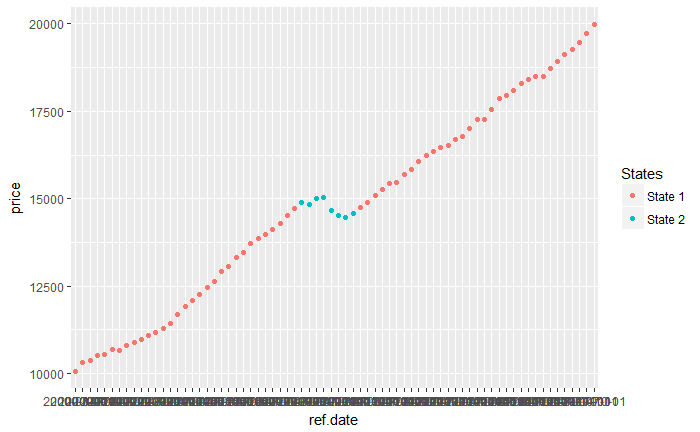
\includegraphics[width=10.5cm,height=6cm,angle=0]{GNP.png}\\
\caption{Regimes by GNP}
\end{figure}

Obviously, using GNP data, the regime switching model can only detect the financial crisis in 2008, with green dots shown on the diagram. For GNP represents the American economy instead of market trend, it is hard to impact the GNP data for normal market crisis, which means the GNP is not sensitive to market crash. So we can hardly use the GNP to detect the crisis in market and give us an insight about the market regime.

\subsection{Regime Switching Model by S\&P 500}
We also implement the regime switching model with S\&P 500 Index, which could offer a better insight on market states. Actually we need to use monthly data in S\&P 500, to match with our bond yield in next section.

\begin{figure}[H]
\centering
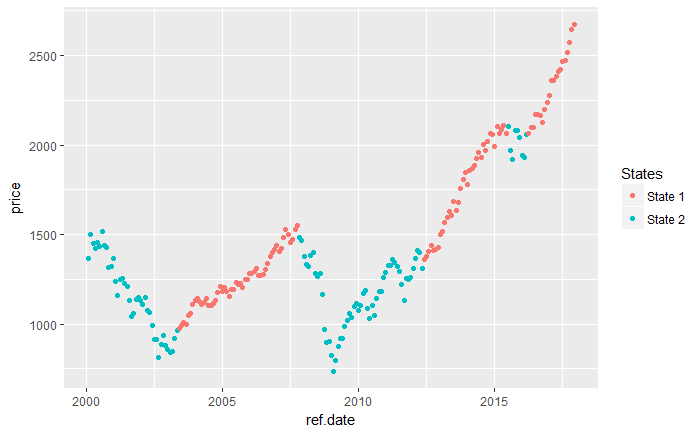
\includegraphics[width=10.5cm,height=6cm,angle=0]{SNPM.png}\\
\caption{Regimes by S\&P 500}
\end{figure}

As what we expected, the S\&P 500 data works as a good indicator for market crisis. From the green dot, we can identify three period of crisis in financial market, the collapse of dot-com bubble at beginning of new century, the financial crisis in 2008 and oil crisis in 2015. The partition works well to identify crisis.\\

For our S\&P 500 monthly return model, the mean return during Normal State is 1.14\% while the model standard deviation is 2.21\%. In Crisis State, the mean return is -0.4\% and the model standard deviation is 5.5\%. The key takeaway we found in almost all of our model is that S\&P 500 monthly return goes up faster in the Normal State than in the crisis state. The return in crisis state is generally negative. Also, the volatility in crisis state is much higher than that in the normal state.\\

Overall, we compare the result of crisis identified by S\&P 500 Index with NBER, which identify the beginning of new century and 2008 are in crisis. So, regimes decideded by the S\&P 500 data are more reasonable compared to the GNP data, so in the next few sections, our analysis will focus more on the S\&P 500 market regimes. 


\pagestyle{fancyplain}
\lhead{\fancyplain{}{\sf Mingcan, Lihua, Duo, Runsheng}}
\rhead{\fancyplain{}{\sf PCA on Fama Bliss Yield}}
\cfoot{}

\section{PCA on Fama-Bliss Yield}

Principal component analysis (PCA) is a
dimension-reduction tool that can be used to
reduce a large set of variables to a small set
that still contains most of the information in
the large set. We assume the Fama-Bliss Yield data are correlated, hence we use PCA to transform the original variables to the linear combination of these variables which are independent. Then we select the number of Principal Components to be considered, given the percentage of variation that we want to be captured in the abridged data set. In this section, we utilize PCA to find the bonds that affect the interest risk the most and extract the contributions of yields with different maturities for later use in the linear regression, which can help us to visualize the other risks embedded in the corporate bonds.\\


 We would like to perform PCA by monthly Fama-Bliss data for holding period returns instead of FRED data, because Fama Bliss bonds are fully taxable and non-callable. Also, since there is missing values in the monthly Fama-Bliss data before Year 2000, we only perform PCA on the Fama-Bliss Yield ranging from 2000 to 2017. For Fama Bliss data with long maturity date are more volatile, we only use 10 types of Treasuries with different maturity in the Fama-Bliss Yield data with relative short-term. 


\subsection{Whole Sample}

We first perform PCA on the Fama-Bliss Treasury yields in the full-period, from 2000 to 2017 and get the 10 PCs.

\begin{figure}[H]
\centering
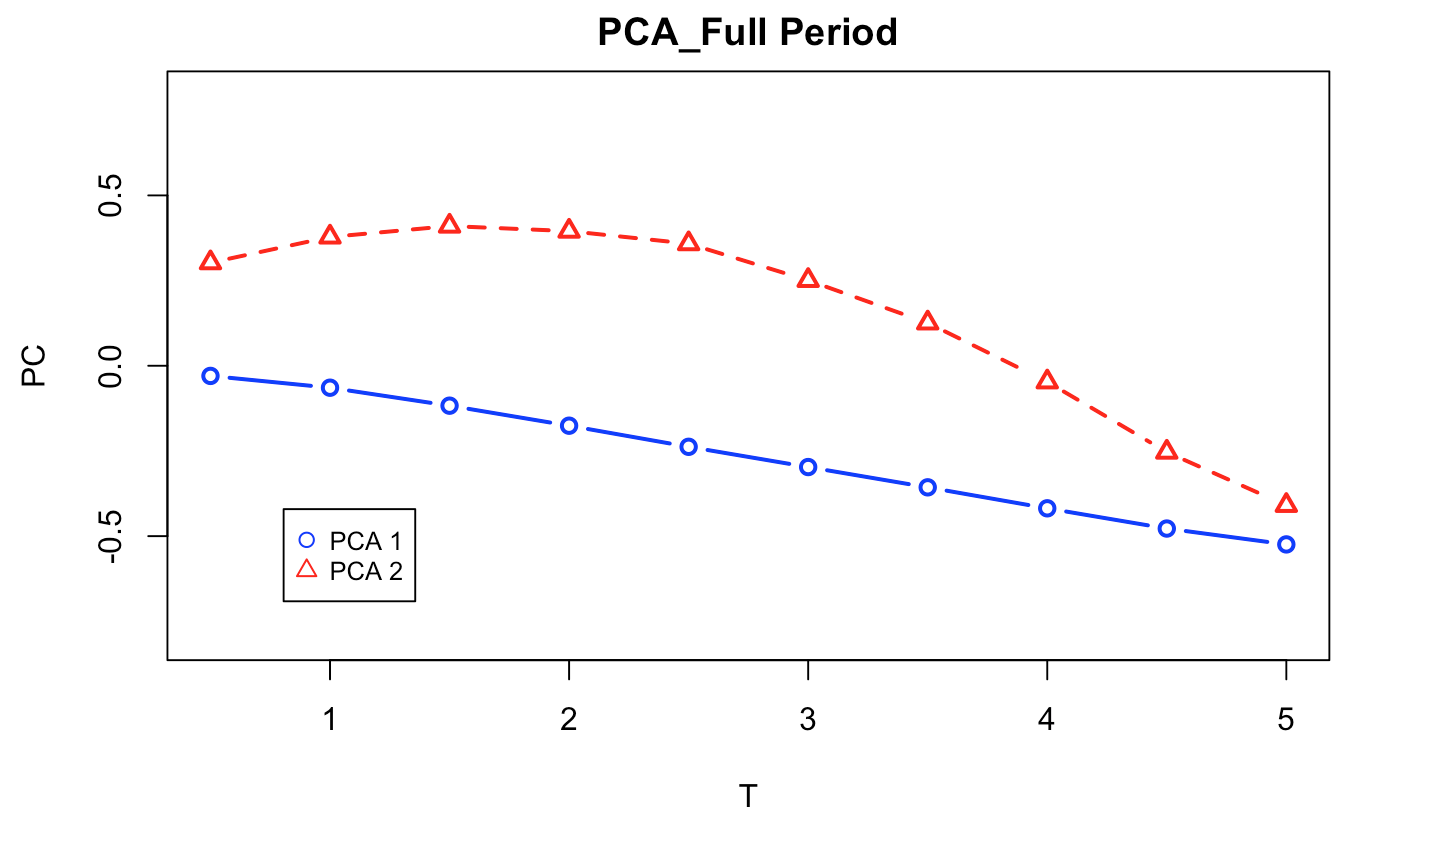
\includegraphics[width=16.5cm,height=9cm,angle=0]{1.png}\\
\caption{PC1 and PC2 Eigen Vectors}
\end{figure}


The result of PCA shows that PC1 and PC2 can explain up to 99\% of the interest rate risk from 2000 to 2017. Also, from the diagram above, we could assert that bond with maturity 3 years to 5 years are the major component of PC1.

\subsection{Different Regimes}

Based on the regime switching model introduced in Section 2, we can split the year 2000 to 2017 into 2 states, the normal and crisis state based on S\&P 500 Index, for S\&P 500 could better reflect the trend of market. We perform PCA on these two state separately to see if there are any difference in the PCs. 


\begin{figure}[H]
\centering
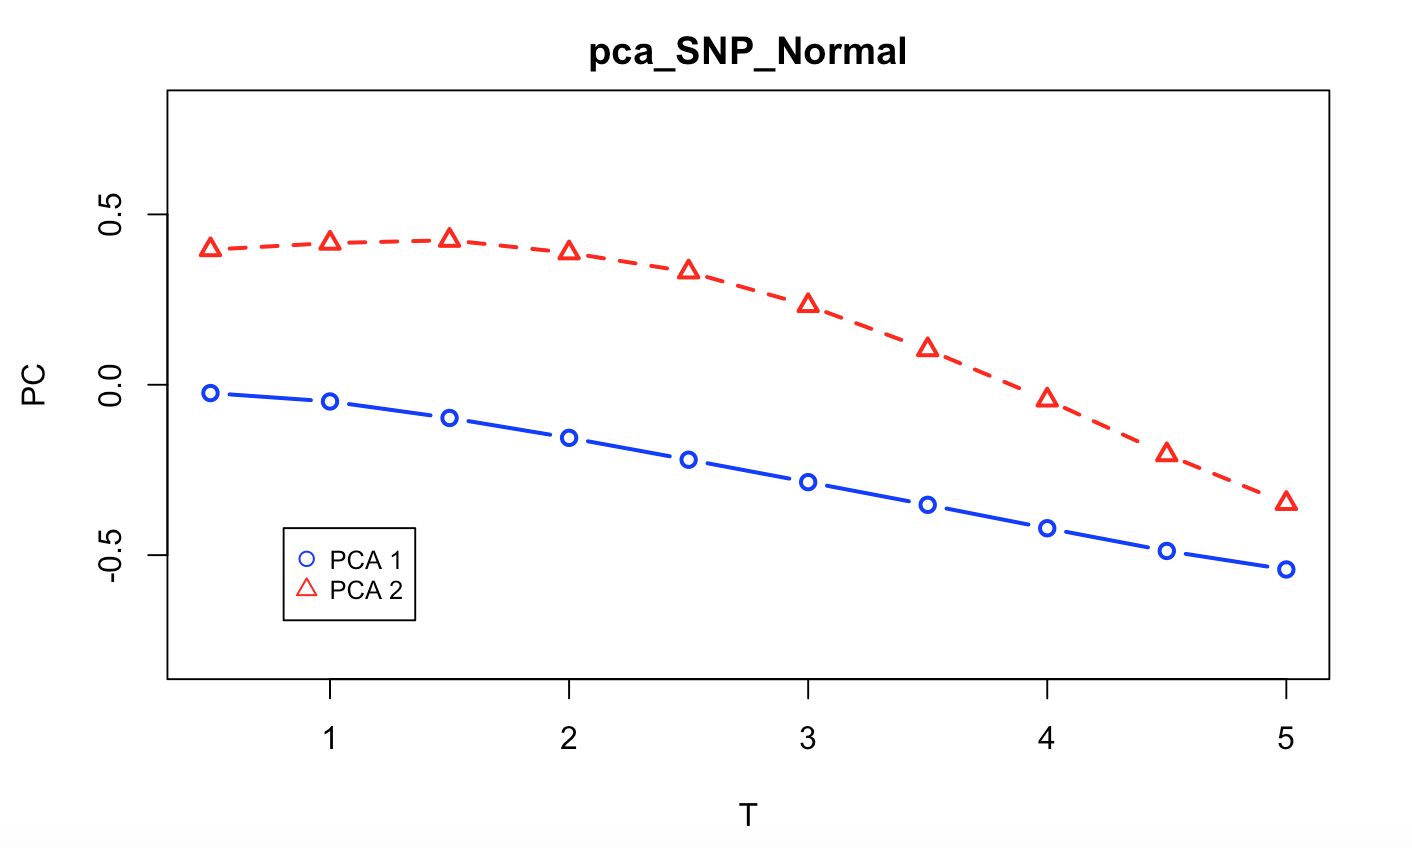
\includegraphics[width=16.5cm,height=9cm,angle=0]{10.png}\\
\caption{PC1 and PC2 Eigenvectors (Normal State)}
\end{figure}


\begin{figure}[H]
\centering
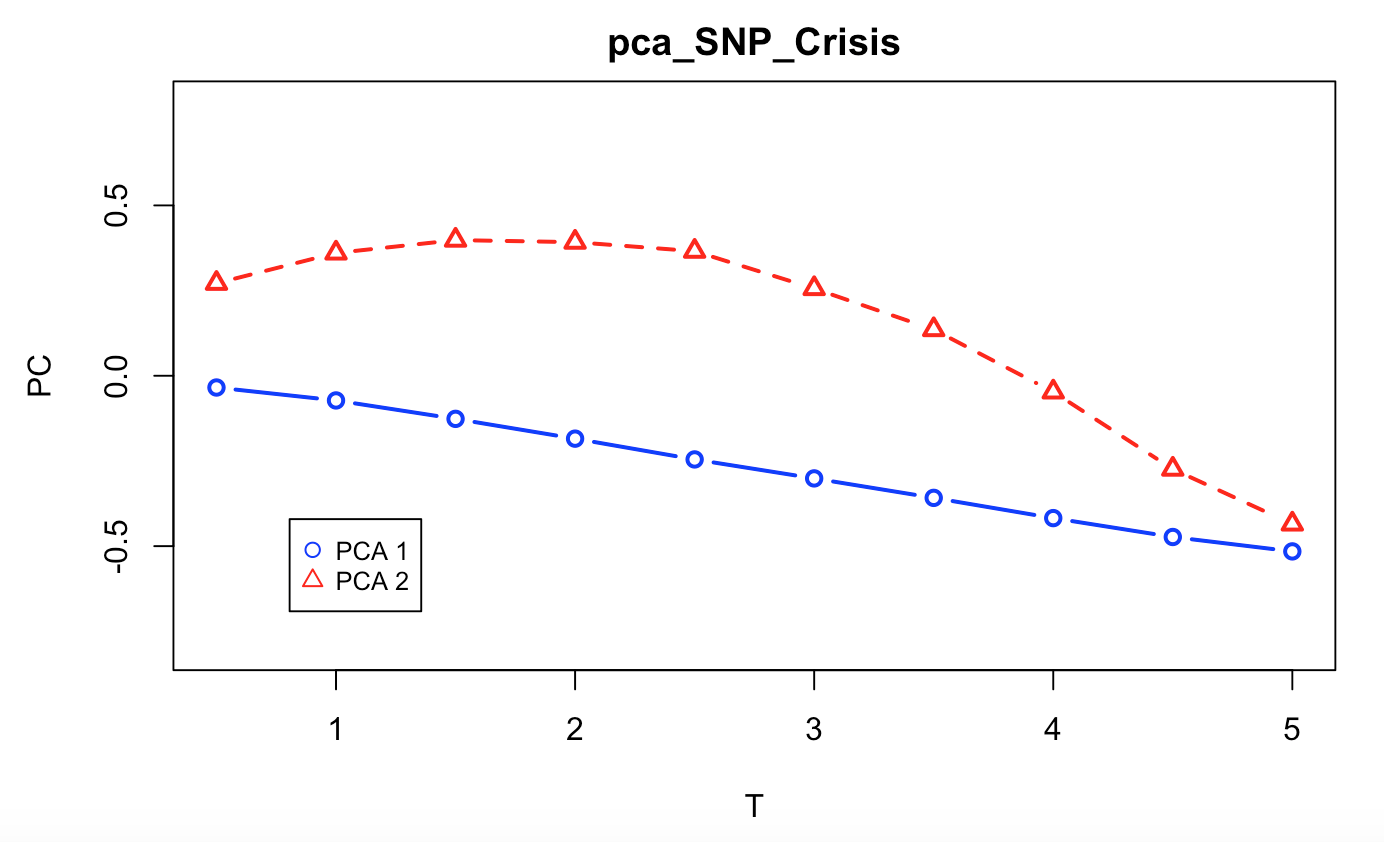
\includegraphics[width=16.5cm,height=9cm,angle=0]{13.png}\\
\caption{PC1 and PC2 Eigenvectors (Crisis State)}
\end{figure}


The PCA results (See appendix) show that PC1 and PC2 can explain up to 99\% of the interest rate risk from 2000 to 2017 in both the normal and crisis state. Also, Bond with maturity 3 years to 5 years have the highest contributions to PC1.

\begin {table}[H]
\caption {PC1 S\&P 500 Regime} 
\label{tab:title} 
\begin{center}
\begin{tabular} {c|c|c|c|c|c|c|c|c|c|c}
\hline\hline
Maturity(year) &0-0.5 &0.5-1 &1-1.5 &1.5-2 &2-2.5 &2.5-3 &3-3.5 &3.5-4 &4-4.5 &4.5-5 \\
\hline
PC1 Normal &-0.024&-0.049&-0.097&-0.156&-0.22&-0.286&-0.352&-0.421&-0.488&-0.542
\\
\hline
PC1 Crisis &-0.034&-0.072&-0.126&-0.184&-0.246&-0.301&-0.358&-0.418&-0.473&-0.504
\\
\hline
Difference &0.0006&0.0028&0.006&0.010&0.012&0.009&0.004&-0.003&-0.014&-0.029
\\
\hline\hline
\end{tabular}\\
\end{center}
\end {table}

Since each entry of PC1 is the major contribution of that corresponding bond to the interest rate risk, in table 1, last row is to investigate the difference in the contribution of each bond in different states. The difference is defined as

$$\textrm{difference}_i=(pc1\_\textrm{normal})_i^2-(pc1\_\textrm{crisis})_i^2 \,\,\,\,\,\textrm{for}\,\,\,\,\,\, i=1,2...10$$ 

Since the last few entries in difference are negative while the rest are positive, we can conclude that under the regime switching based on S\&P 500 data, the long-term bond could represent more variance in interest rate risk in normal state and the the short-term bond could represent more variance in interest rate risk in crisis state.\\


Overall, since there is not much difference in the PCs and the general pattern of variance explained, for the rest of the project, and the regime switching model shows the S\&P 500 regimes are more reasonable, we will stick to use the PC1 and PC2 generated from different regimes under S\&P 500. \\




\pagestyle{fancyplain}
\lhead{\fancyplain{}{\sf Mingcan, Lihua, Duo, Runsheng}}
\rhead{\fancyplain{}{\sf Regressions}}
\cfoot{}

\section{Regressions}

As we mentioned above, we perform PCA on Fama-Bliss yields with different maturities and get the principal components. We can see that the first two principal components can explain more than 99\% variance in the whole sample, the normal state and the crisis state. In this section, we would perform linear regressions on the ICE BofAML US Corporate Effective Yields with different credit ratings (AAA, BB and CCC), and see whether the two principal components of the Fama-Bliss yields can explain the interest rate risk of these corporate bond yields. We would also analyze the residuals of the regressions because the residuals represent the residual risks of the corporate bond after eliminating the interest rate risk. The residual risks mainly contain the credit risk of the corporate bonds.

\subsection{Regressions on the Whole Sample}

We first regress the three corporate bond yields with credit ratings AAA, BB and CCC respectively on the first two principal components of the Fama-Bliss yields in the whole sample. The regression formula is

$$Y_t = \alpha + \beta_1 PC1_t + \beta_2 PC2_t + \epsilon_t$$

\noindent The table below shows the regression results. 


\begin {table}[H]
\caption {Regression results in the whole sample} 
\label{tab:title} 
\begin{center}
\begin{tabular} {c c c c}
\hline\hline
Variables & AAA & BB & CCC \\
\hline

\multirow{$\alpha$} & 0.0332*** & 0.063*** & 0.132*** \\
                    & (36.63) & (39.92) & (28.26) \\

\multirow{PC1} & -0.138*** & -0.304*** & -0.734*** \\
               & (-4.12) & (-5.20) & (-4.23) \\

\multirow{PC2} & 2.169*** & 1.914*** & 4.086*** \\
               & (12.11) & (6.12) & (4.41) \\
\hline

$R^2$ & 0.436 & 0.233 & 0.15 \\

\hline\hline

\end{tabular}\\

\noindent t statistics in parentheses \\

\noindent *** $p < 0.01$, ** $p < 0.05$, * $p < 0.1$
\end{center}
\end {table}


\subsection{Regressions in Different Regimes}

We regress the three corporate bond yields on the first principal components in the normal period that is determined by the Markov switching model on the S\&P 500 monthly return. Note that the principal components here are different from those computed in the whole sample. The regression form is

$$Y_t = \alpha + \beta_1 PC1_t^{(normal)} + \beta_2 PC2_t^{(normal)} + \epsilon_t$$

\noindent where $t$ is the time in the normal period. 

\noindent The table below shows the regression results. 


\begin {table}[H]
\caption {Regression Results in Normal State} 
\label{tab:title} 
\begin{center}
\begin{tabular} {c c c c}
\hline\hline
Variables & AAA & BB & CCC \\
\hline

\multirow{$\alpha$} & 0.029*** & 0.051*** & 0.110*** \\
                    & (27.70) & (53.17) & (58.40) \\

\multirow{PC1} & -0.073 & -0.0980** & 0.029 \\
               & (-1.57) & (-2.34) & (0.35) \\

\multirow{PC2} & 2.816*** & 2.515*** & 0.286 \\
               & (10.35) & (10.26) & (0.60) \\
\hline

$R^2$ & 0.504 & 0.506 & 0.004 \\
\hline\hline

\end{tabular}\\

\noindent t statistics in parentheses \\

\noindent *** $p < 0.01$, ** $p < 0.05$, * $p < 0.1$
\end{center}
\end {table}


Also, we can regress the three corporate bond yields on the first two principal components in the crisis period. The regression form is 

$$Y_t = \alpha + \beta_1 PC1_t^{(crisis)} + \beta_2 PC2_t^{(crisis)} + \epsilon_t$$
\noindent where $t$ is the time in the normal period. 

\noindent The table below shows the regression results. 


\begin {table}[H]
\caption {Regression Results in Crisis State} 
\label{tab:title} 
\begin{center}
\begin{tabular} {c c c c}
\hline\hline
Variables & AAA & BB & CCC \\
\hline

\multirow{$\alpha$} & 0.037*** & 0.078*** & 0.171*** \\
                    & (24.71) & (32.22) & (22.91) \\

\multirow{PC1} & -0.127*** & -0.202** & -0.529** \\
               & (-2.65) & (-2.58) & (-2.20) \\

\multirow{PC2} & 1.926*** & 1.419*** & 4.596*** \\
               & (8.07) & (3.64) & (3.84) \\

\hline 

$R^2$ & 0.417 & 0.165 & 0.162 \\
\hline\hline

\end{tabular}\\

\noindent t statistics in parentheses \\

\noindent *** $p < 0.01$, ** $p < 0.05$, * $p < 0.1$
\end{center}
\end {table}


\subsection{Results Analysis}

From the results of the three regressions in different market regimes, the significant coefficients show that the principal components of Treasury yields can mostly explain the interest rate risk of the three corporate bond yields in the whole sample, normal and crisis period. There is only one exception, that is, for the CCC yields, the coefficients are not significant in the normal period and the $R^2$ is small.\\

We further analyze the residuals of the regressions. The residuals of the regression actually can represent the other risks except the interest rate risk of the corporate bonds. The major risk in the residuals is the credit risk. Thus, we can explore the residuals to analyze the credit risk premium of the bond. \\

We performed some tests on the residuals. We attached all the test plots in the appendix. First, we tested the auto-correlations of the residuals by the acf plot in R. From the acf plot, we can see that the residuals have significant auto-correlations. These may cause some bias in the coefficients of the regression, but we still kept our analysis because the model has its own economic sense. Then we tested the normality of the residuals. We can see that the AAA bond residuals appear normal in different market regimes. The BB and CCC bond residuals have slightly heavy right tail in the crisis period, which corresponds to high credit risk premium in the crisis period. \\

Then we plot the residuals of different market regimes in the same figure to compare credit risk premium. We can see a pattern in the figures. The residuals in the crisis period are slightly lower than those in the whole sample, while the residuals in the normal period are slightly higher than those in the whole sample. Our explanation is that people are willing to pay more credit premiums in the crisis period compared to the true credit risk premium, while they pay less credit premiums in the normal period. In the real world, people may find it hard to distinguish the normal and crisis period, so the residuals in the whole sample can represent the credit risk premiums that people actually paid. However, the credit risk premiums in the crisis period may be represented more accurately by the residuals in the crisis period because the residuals are obtained only in the crisis period. This argument can still be applied in the normal period.

\begin{figure}[H]
\centering
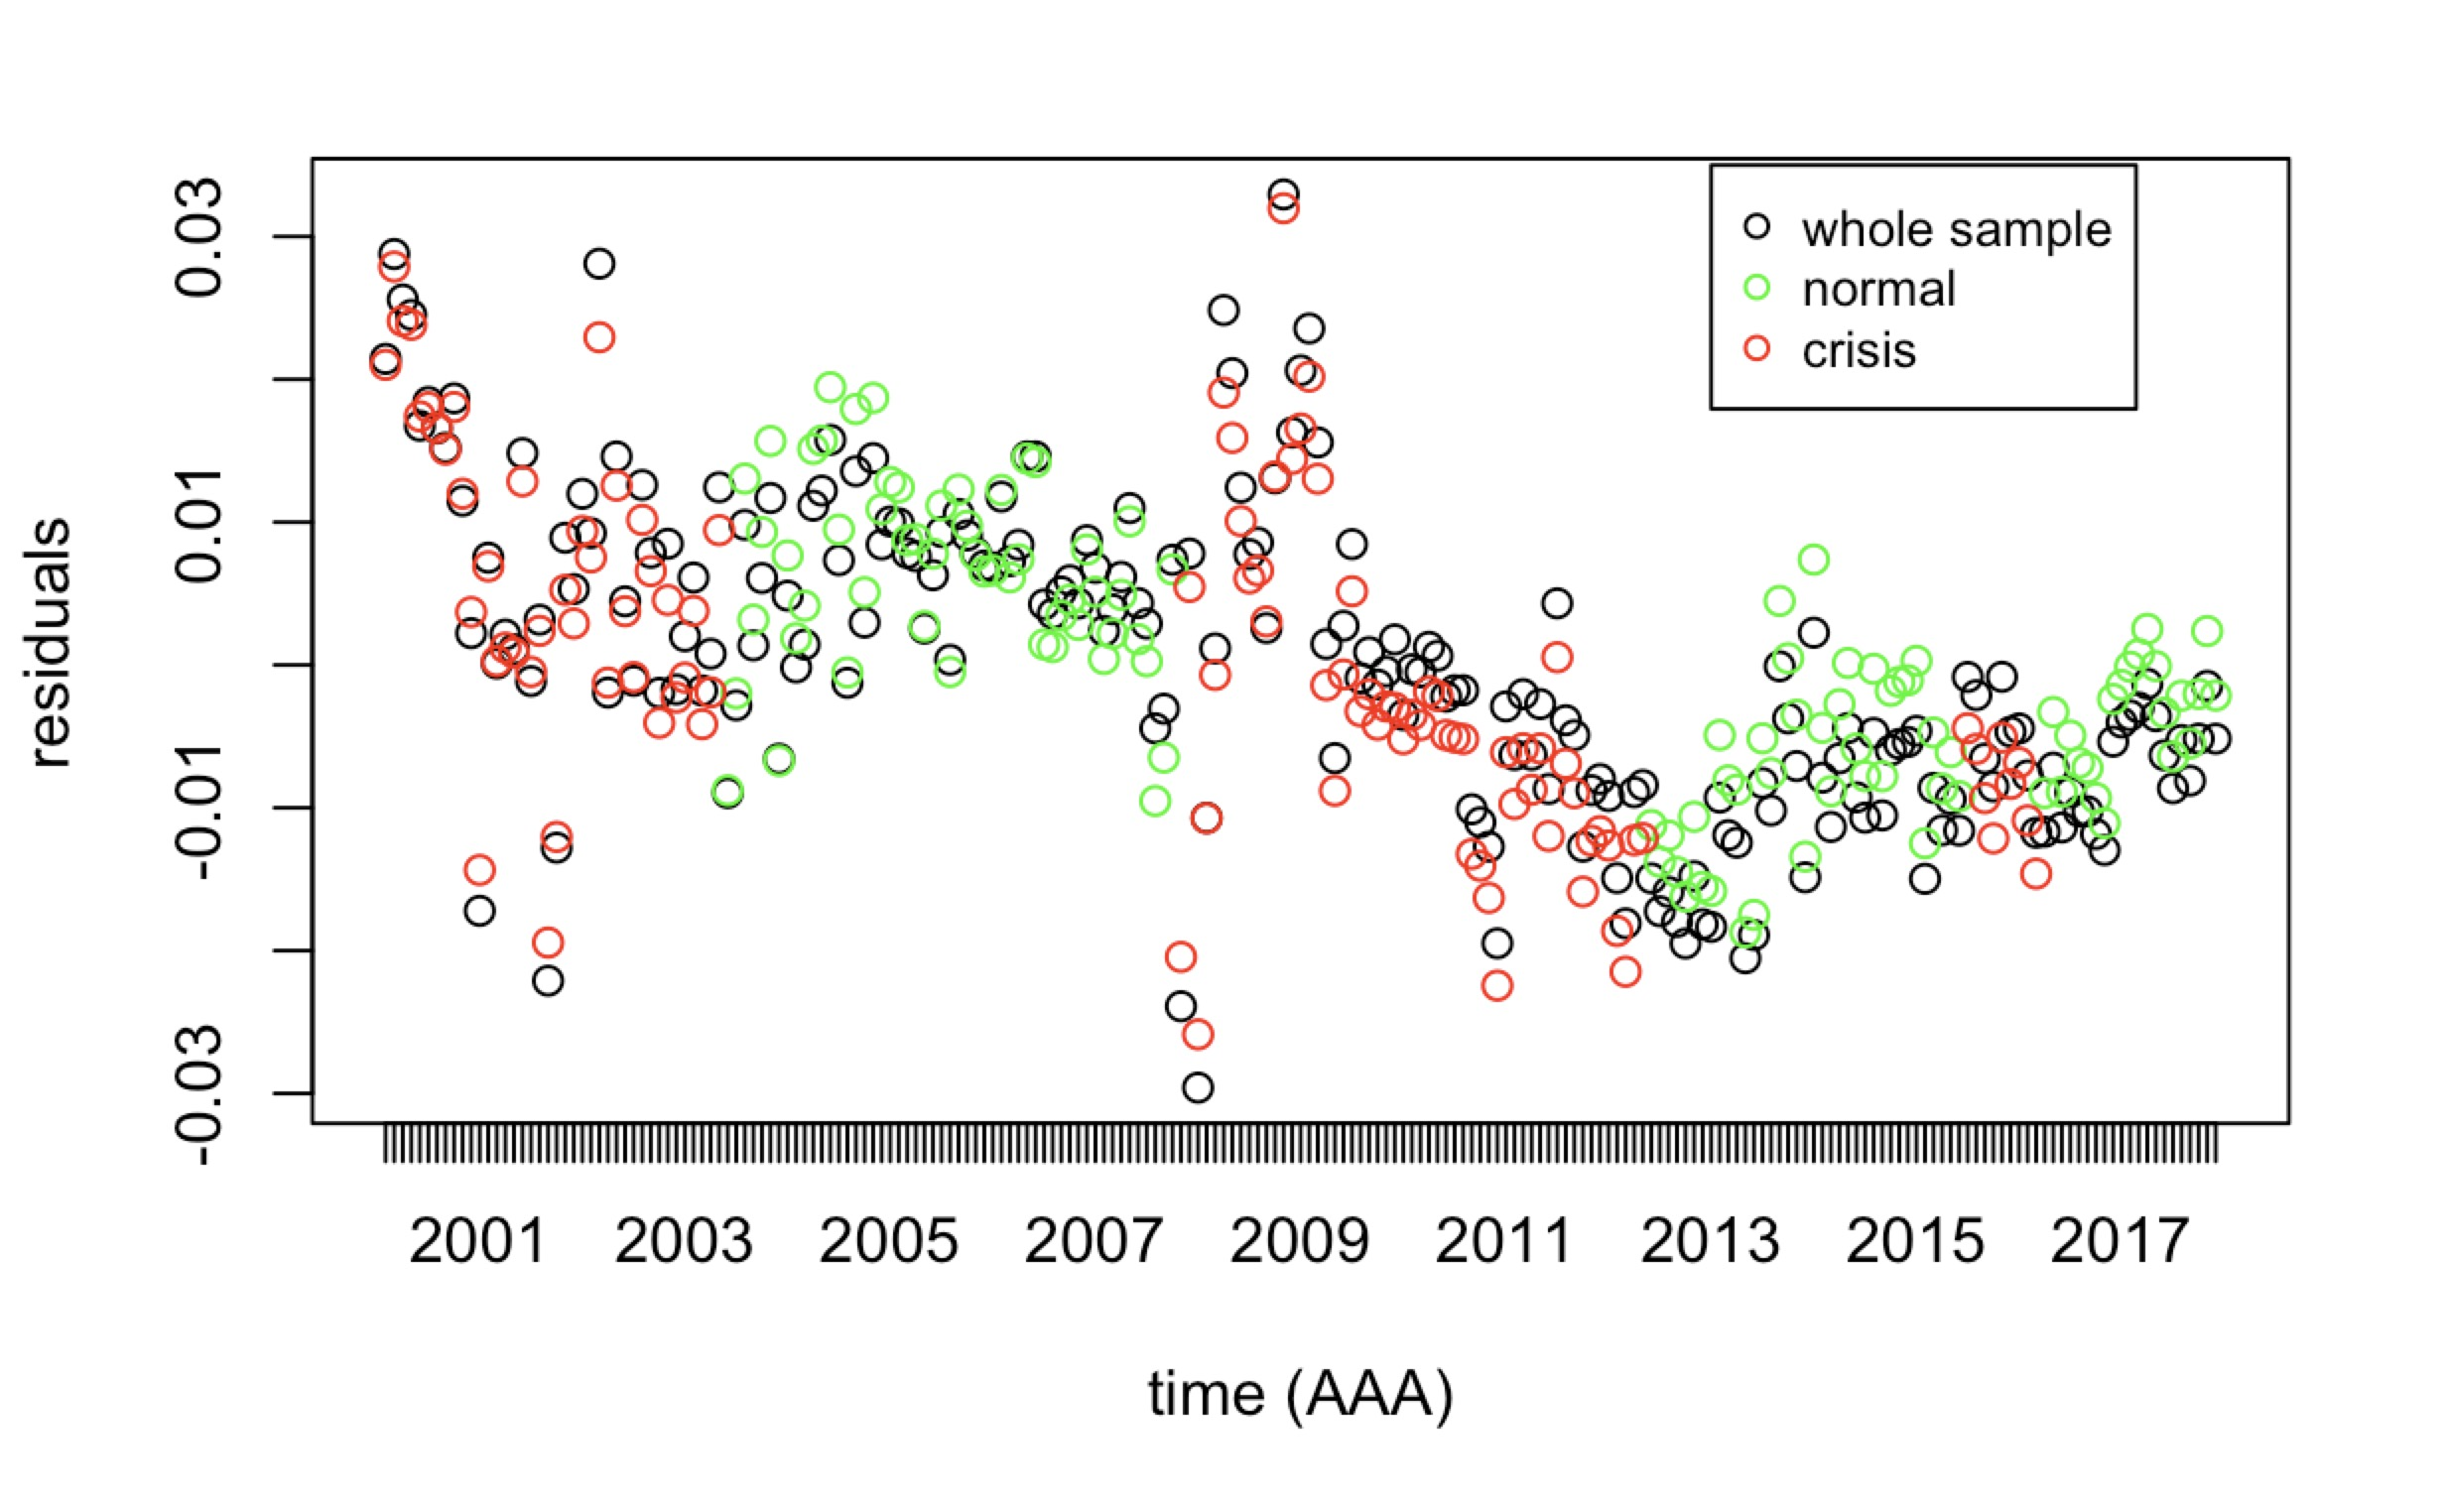
\includegraphics[width=16.5cm,height=8.5cm,angle=0]{AAA_resid_comparison.jpg}\\
\caption{AAA Bond Residuals}
\end{figure}

\begin{figure}[H]
\centering
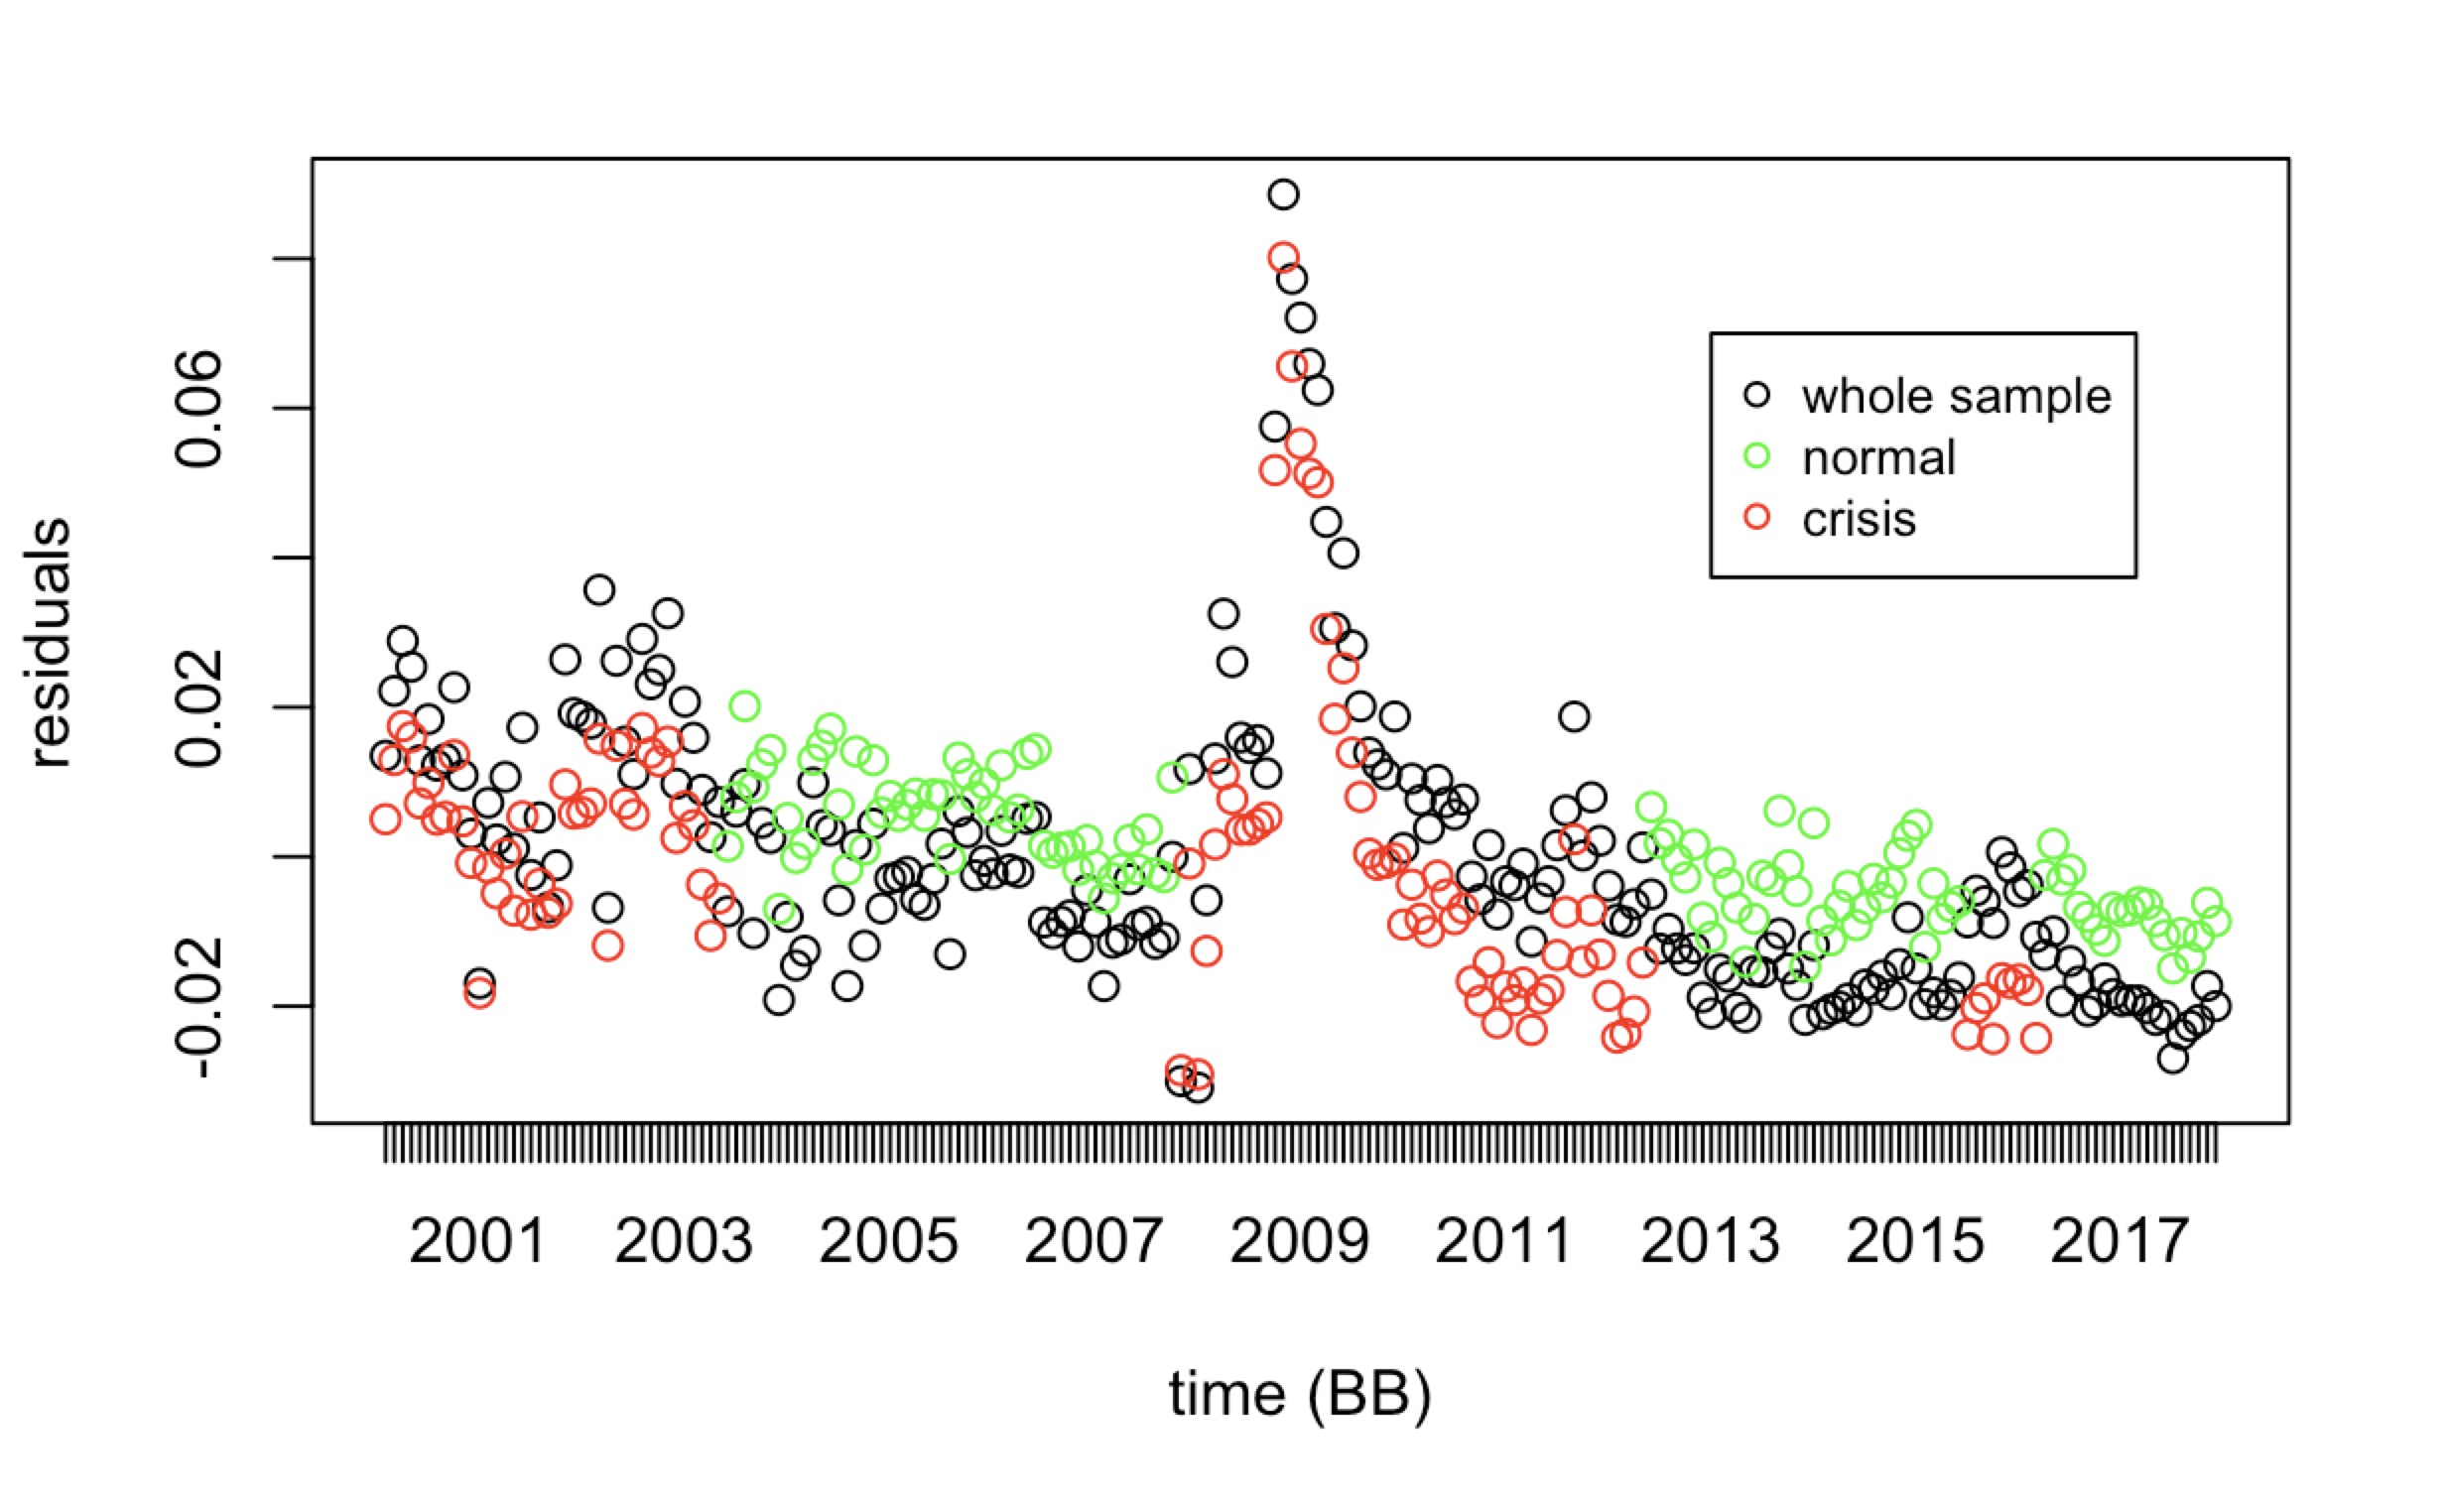
\includegraphics[width=16.5cm,height=8.5cm,angle=0]{BB_resid_comparison.jpg}\\
\caption{BB Bond Residuals}
\end{figure}

\begin{figure}[H]
\centering
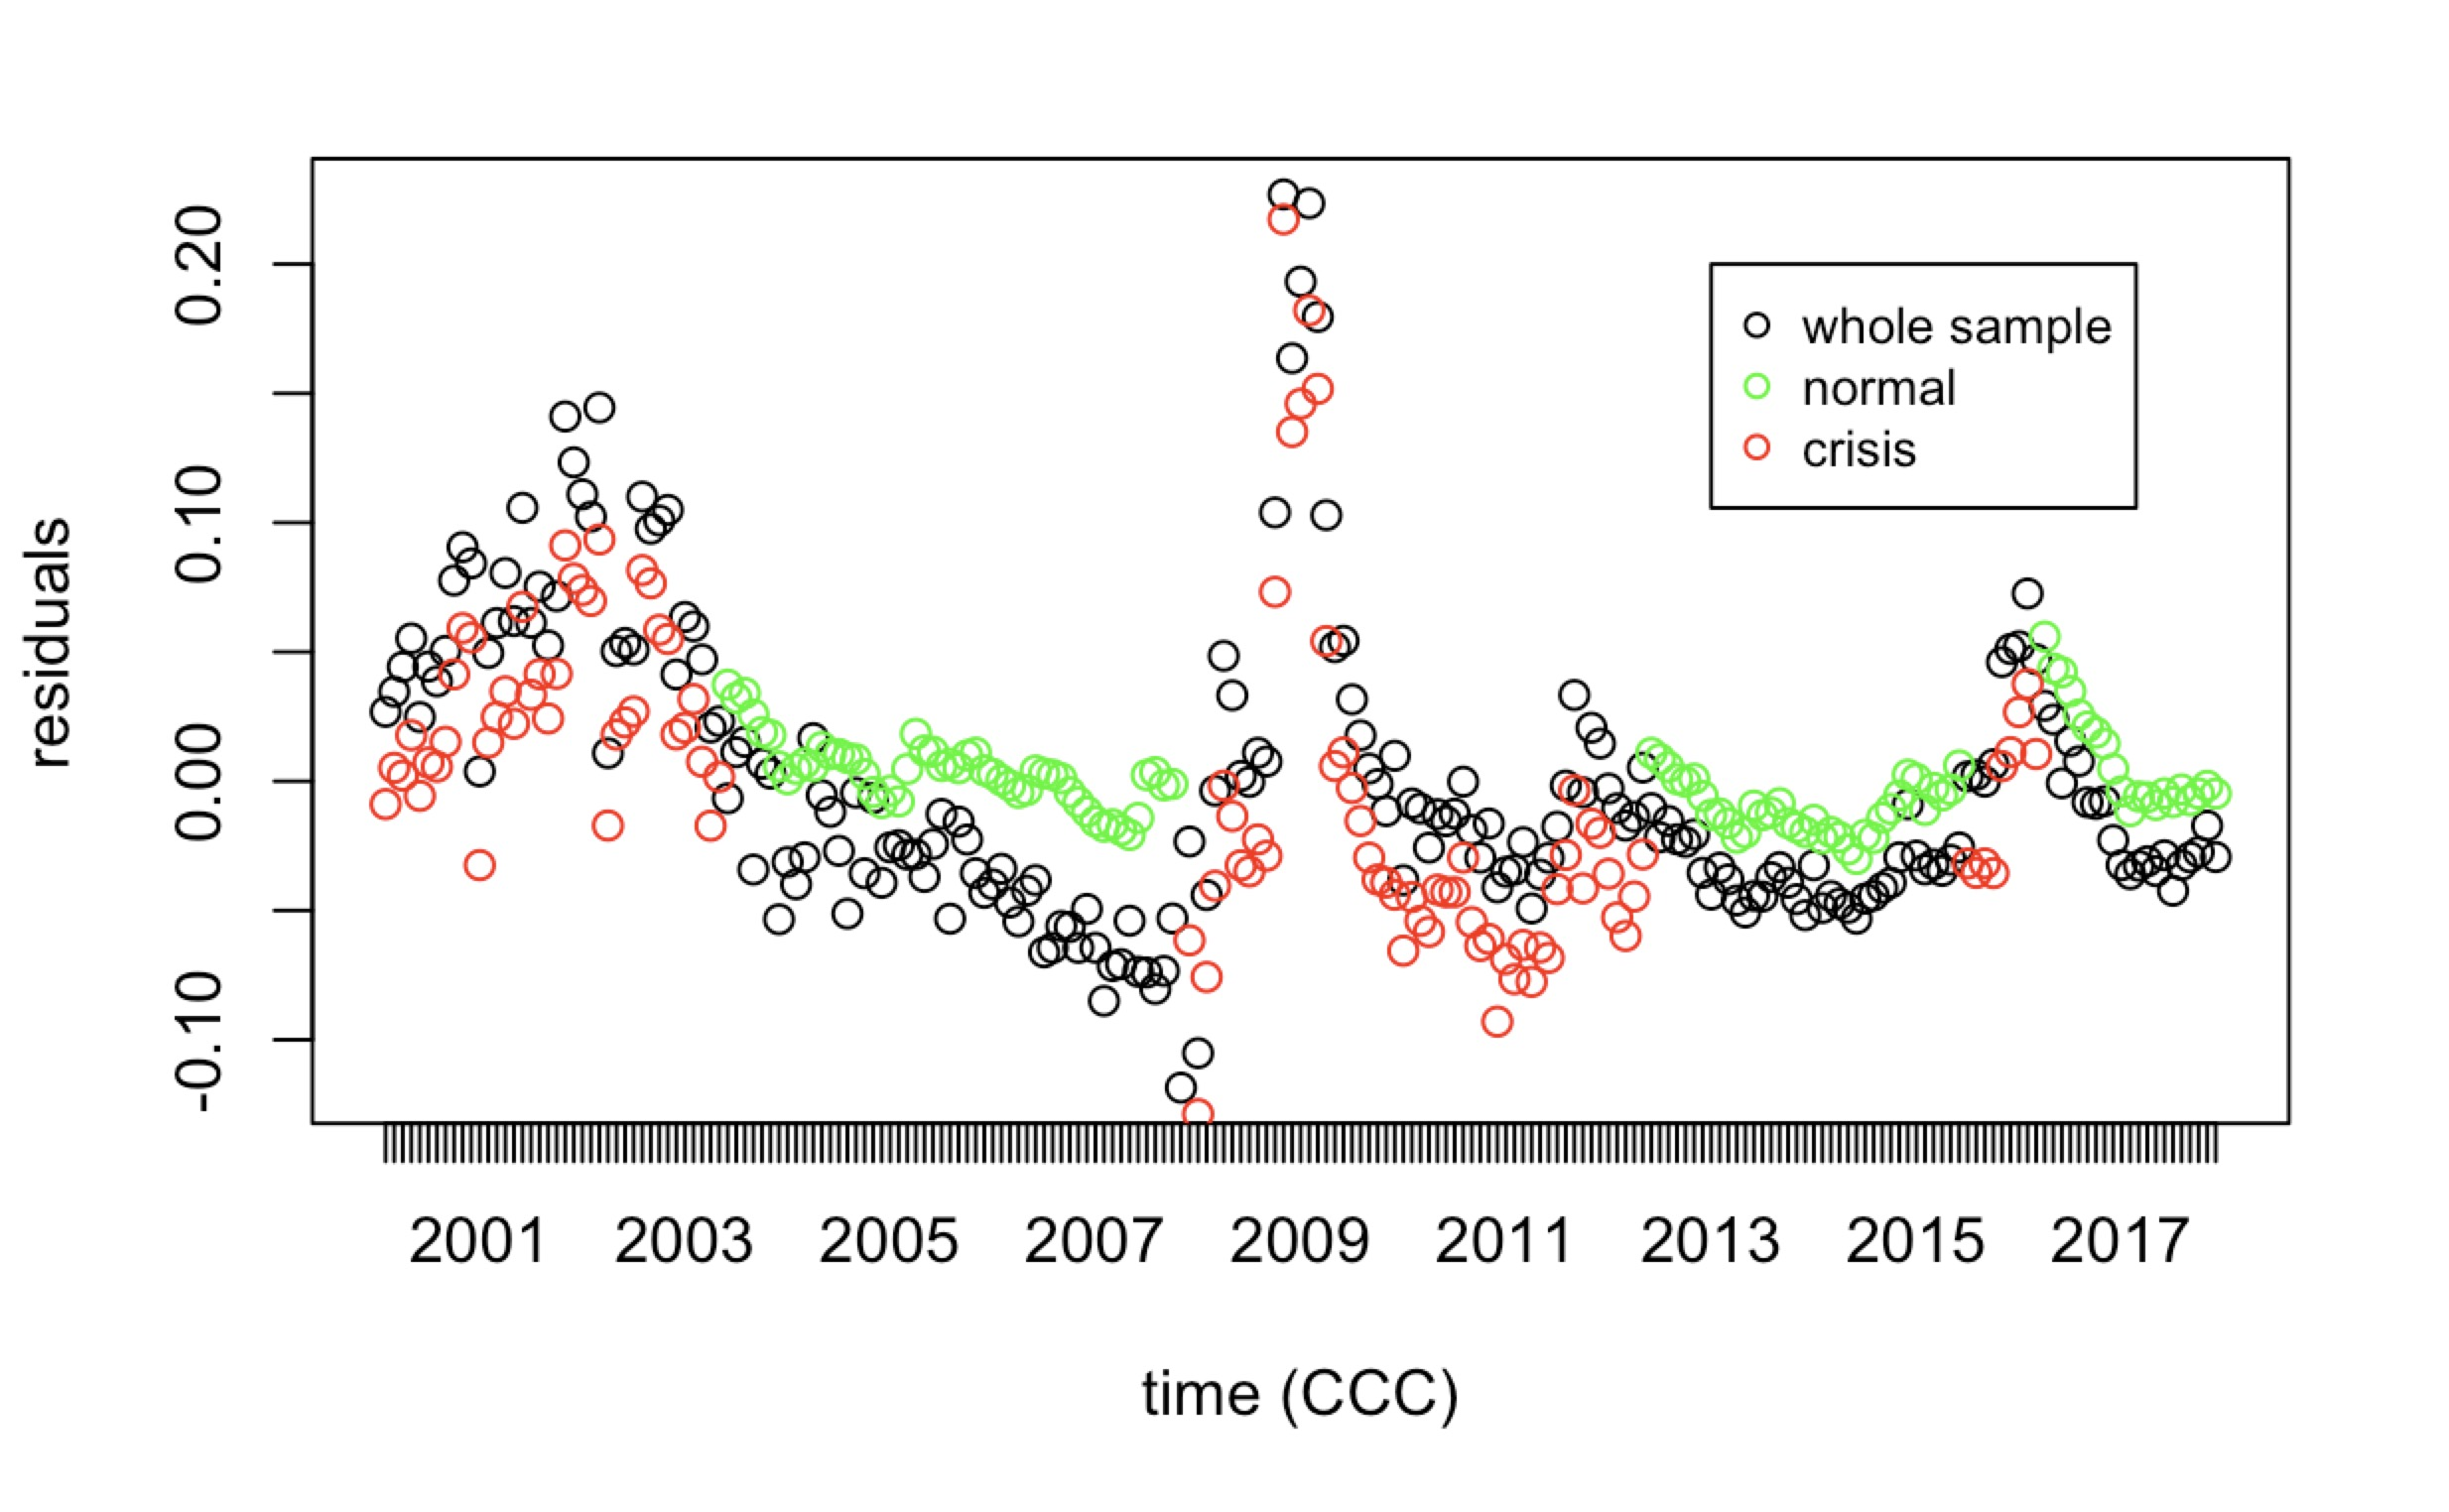
\includegraphics[width=16.5cm,height=8.5cm,angle=0]{CCC_resid_comparison.jpg}\\
\caption{CCC Bond Residuals}
\end{figure}


\subsection{Regressions of the Market Portfolio}

We used S\&P 500 Index as the market portfolio, and projected the market portfolio returns on the first two principal components in the whole sample, the normal and crisis period. The regression forms are

$$R_t = \alpha + \beta_1 PC1_t + \beta_2 PC2_t + \epsilon_t$$

$$R_t = \alpha + \beta_1 PC1_t^{(normal)} + \beta_2 PC2_t^{(normal)} + \epsilon_t$$

$$R_t = \alpha + \beta_1 PC1_t^{(crisis)} + \beta_2 PC2_t^{(crisis)} + \epsilon_t$$

The regression results are shown below.

\begin {table}[H]
\caption {Regression Results} 
\label{tab:title} 
\begin{center}
\begin{tabular} {c c c c}
\hline\hline
Variables & Whole Sample & Normal & Crisis \\
\hline

\multirow{$\alpha$} & 0.012*** & 0.012*** & 0.011* \\
                    & (3.63) & (4.60) & (1.76) \\

\multirow{PC1} & 0.696*** & 0.191* & 0.920*** \\
               & (5.88) & (1.72) & (4.63) \\

\multirow{PC2} & -0.655 & -0.005 & -0.467 \\
               & (-1.04) & (-0.01) & (-0.47) \\
\hline
$R^2$          & 0.144 & 0.0267 & 0.177 \\

\hline\hline

\end{tabular}\\

\noindent t statistics in parentheses \\

\noindent *** $p < 0.01$, ** $p < 0.05$, * $p < 0.1$
\end{center}
\end {table}

The results show that only the first principal components of the Treasury yields is significant in different market regimes. The residual plot below shows that there are no significant difference in the residual risks between different market regimes. We think the reason is the stock market is different from corporate bond market. In addition to interest rate risk, there are many other risk sources associated with the stock market. 


\begin{figure}[H]
\centering
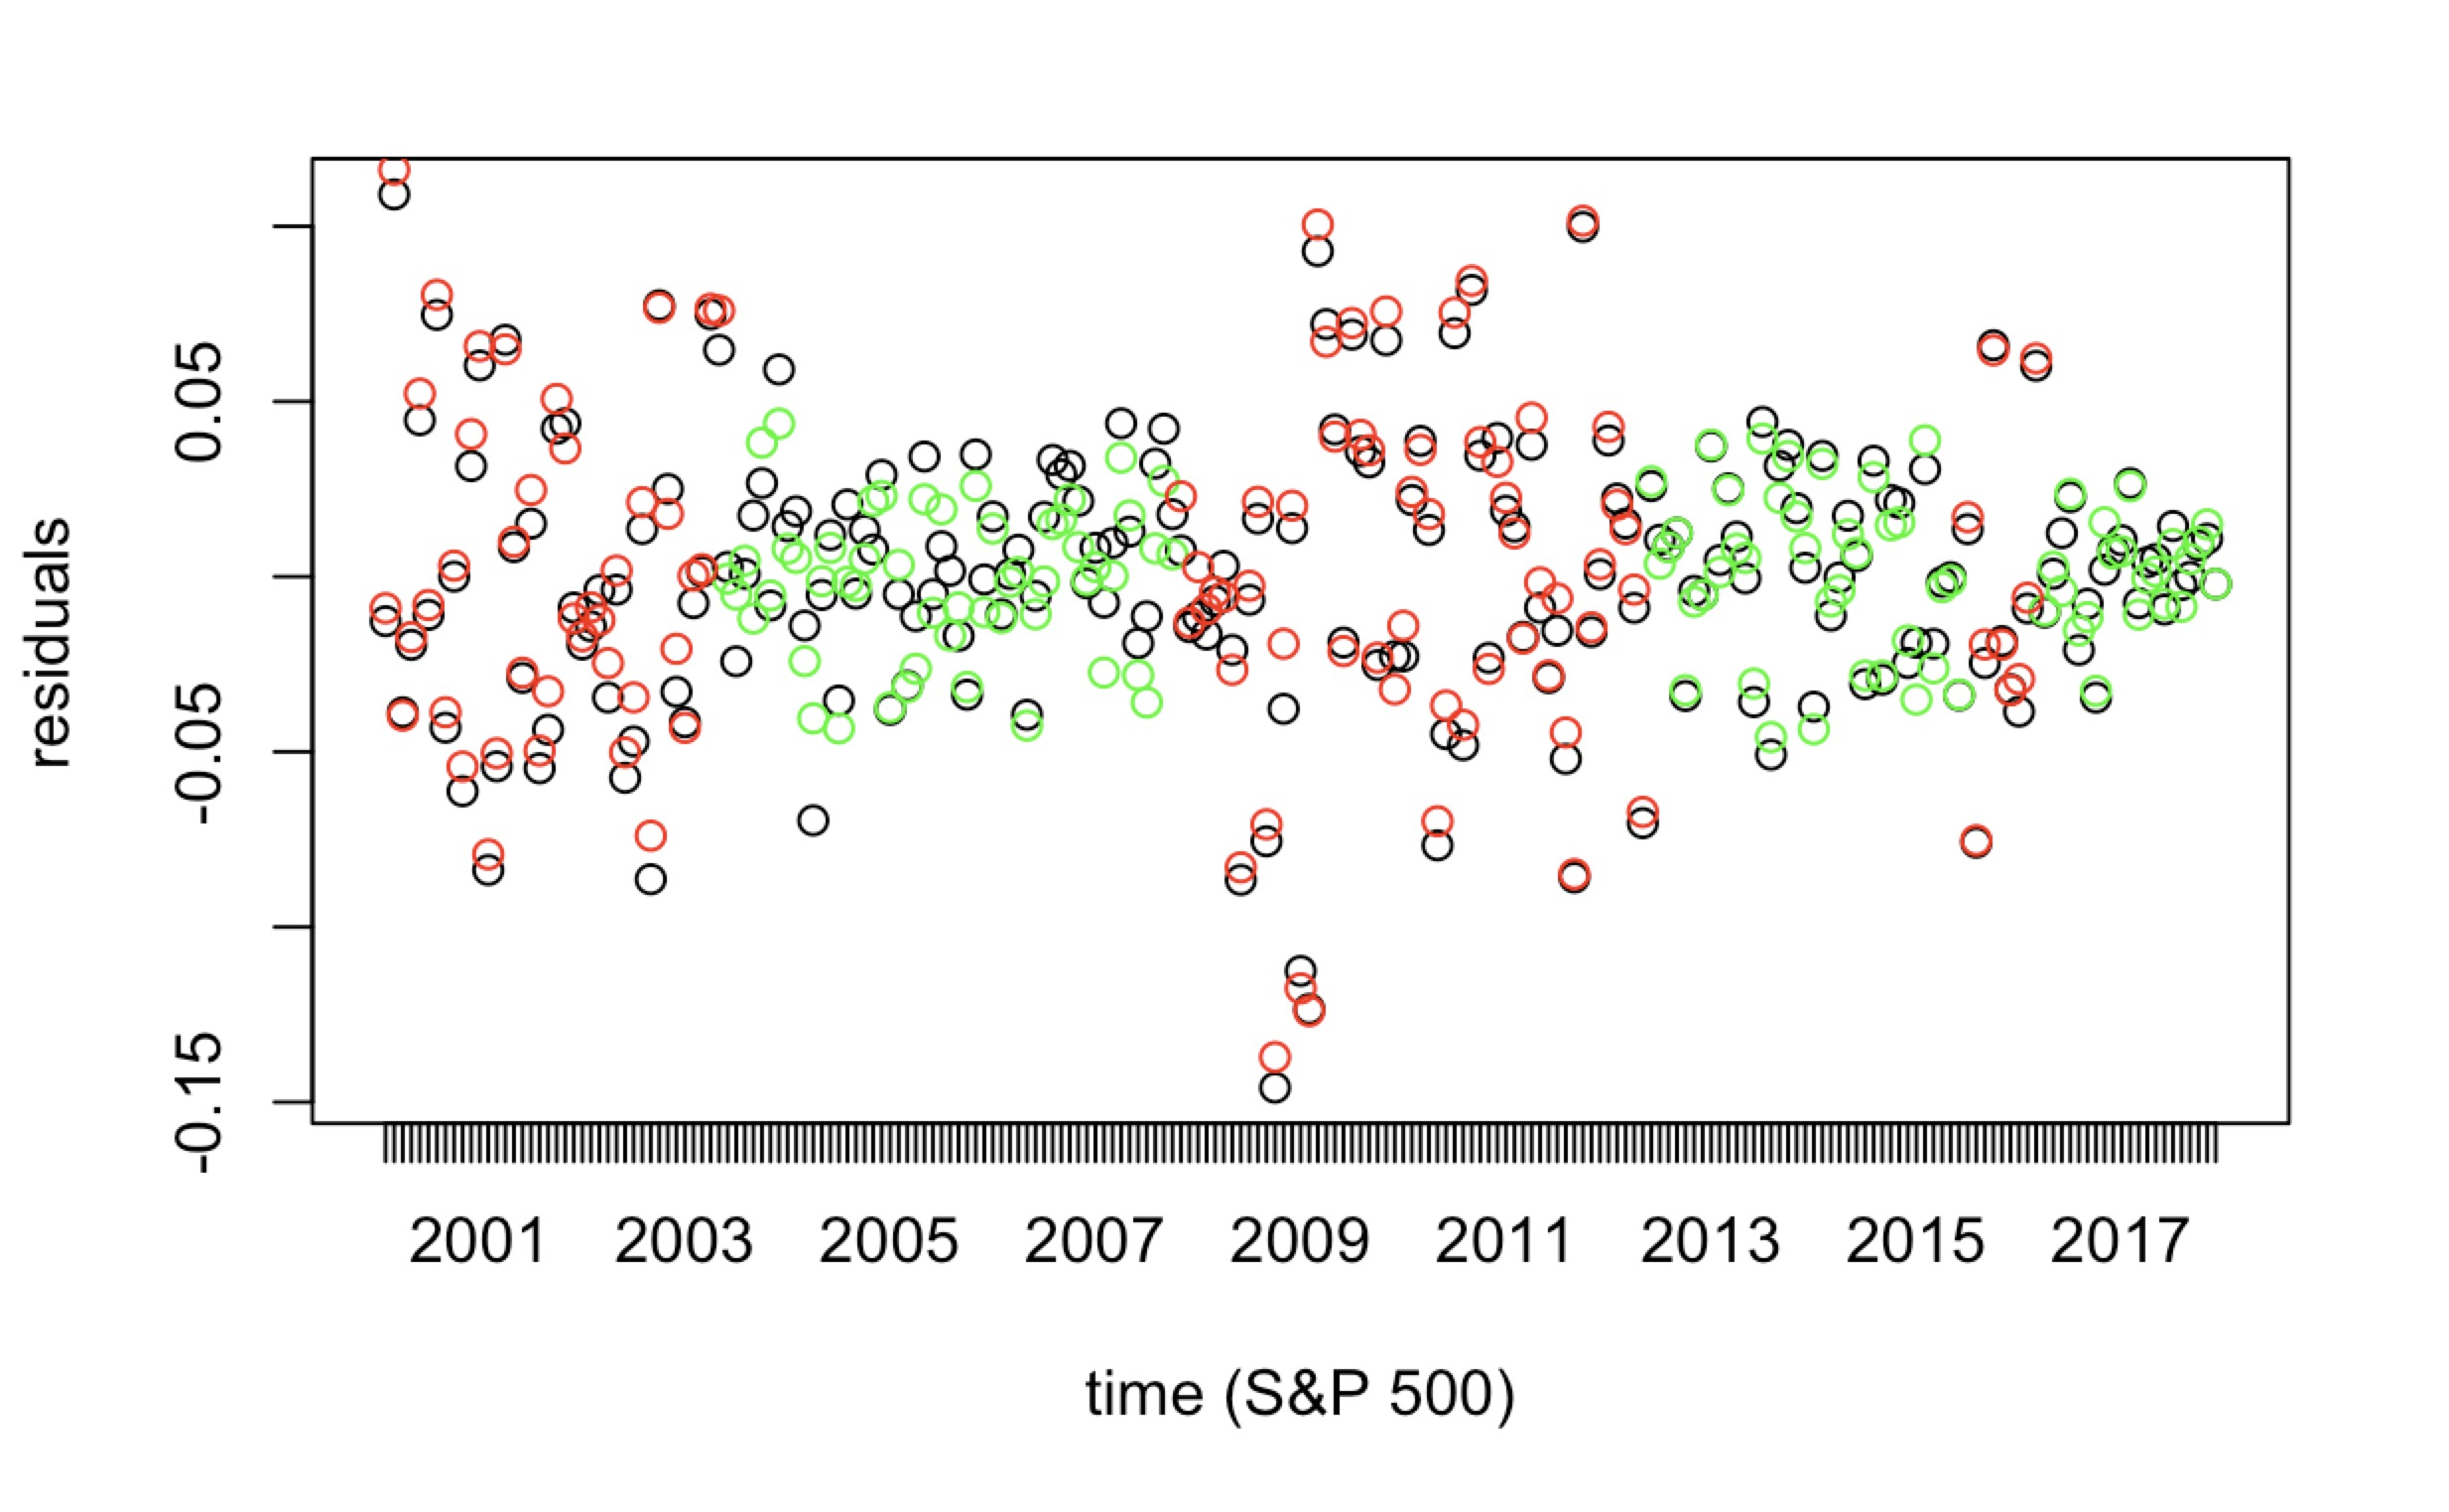
\includegraphics[width=16.5cm,height=8.5cm,angle=0]{s&p500_resid_comparison.jpg}\\
\caption{Market Portfolio Residuals}
\end{figure}





\pagestyle{fancyplain}
\lhead{\fancyplain{}{\sf Mingcan, Lihua, Duo, Runsheng}}
\rhead{\fancyplain{}{\sf Strategy and Portfolio}}
\cfoot{}

\section{Strategy and Portfolio}

In this section, we want to use the results from linear regression and PCA to construct our strategy and portfolio, to catch the credit risk in different period and get the risk premium to make profit. As we have mentioned above, we can quantify the credit risk as residual and intercept, when regress bond price, such as AAA bond, against interest rate and Fama-Bliss yield. And we call the portfolio as credit portfolio \\

In order to construct credit portfolio, we assign weights for each Fama Bliss bond by the sum of weights in PC1 and PC2. As for the bond with maturity at time $i$, after regressing AAA bonds against Fama Bliss yield, we assign bond with the weight at $weight_i$ if we have one AAA bond:

$$
weight_i = -(\beta_1\times(weight\ of\ i\ in\ PC1) + \beta_2\times(weight\ of\ i\ in\ PC2))
$$

When $weight_i$ is positive, it means we need to long $weight_i$ of bond with maturity at time $i$ with every one AAA bond, and when $weight_i$ is negative, it means we need to short $|weight_i|$ of bond with maturity at time $i$ with every one AAA bond. Obviously, in different period, PCA would output different component, and we would construct different portfolio in normal state or crisis state, which make sense that investors should obtain different risk preference in different period.\\

So we can construct credit portfolio for AAA, BB and CCC bond using regime switching model and PCA, analyze the effect of regime switching model and trend of credit crisis in the past decades.

\subsection{AAA bond}
For AAA bond, the weight for each bond portfolio with different maturity day, from Fama Bliss yield, is shown below. The blue bars represent weights for each bond in normal state, the red bars represent the weights for each bond in crisis state, and the green bars are for the weights when using whole sample instead of regime switching model.
\begin{figure}[H]
\centering
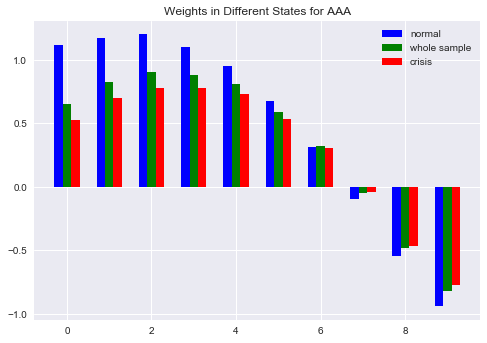
\includegraphics[width=16.5cm,height=6cm,angle=0]{AAA_weight.png}\\
\caption{Weights for bond in AAA}
\end{figure}
As what we expected, the whole sample weights is between the weights from normal state and crisis state. Investors are always willing to long the short-term bonds and short long-term bonds if they need to catch interest rate.\\

Based on the weight, we could long the AAA bond and short the portfolio above, to obtain the credit premium, which is shown below.

\begin{figure}[H]
\centering
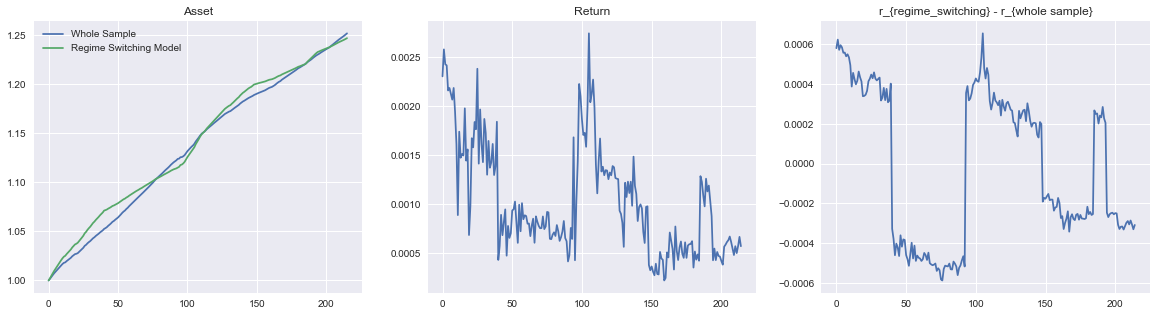
\includegraphics[width=16.5cm,height=5cm,angle=0]{AAA.png}\\
\caption{Credit Portfolio for AAA}
\end{figure}

 Using the diagram on the left, we can find that, for AAA bond, regime switching model didn't improve the performance for credit portfolio, which may be explained by the low sensitivity of AAA bond toward market. From the diagram in the center, the return of credit portfolio of AAA bond shows high correlation with the market. We can see that the return of portfolio goes up when market crashed in 2008 and 2015, which means the risk premium increase with crisis and we can catch it with our credit portfolio. The diagram on the right shows the difference of return when using regime switching model, that regime switching didn't work well for AAA bond and sometimes even under performed. 

\subsection{BB bond}
For BB bond, we could regard it as Junk Bond. Intuitively, it would perform differently against the AAA bond. We can see the weights for each bond in order to hedge interest risk in BB bond as below.
\begin{figure}[H]
\centering
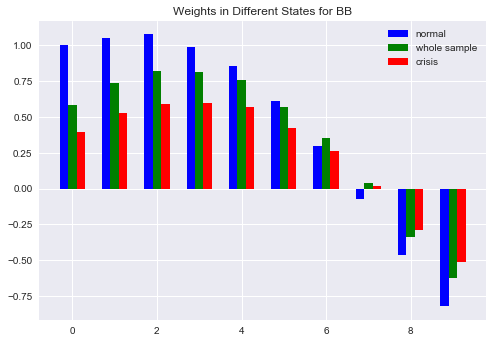
\includegraphics[width=16.5cm,height=6cm,angle=0]{BB_weight.png}\\
\caption{Weights for bond in BB}
\end{figure}
Obviously, the gap between height of blue bar and red bar becomes larger, which means the BB bond requires us to hold the significantly different bond portfolio for normal and crisis period, when hedging the interest rate risk in BB bond. Moreover, we still long the short-term bonds and short long-term bonds in order to represent the interest rate risk.\\

Then, we can check the performance of credit portfolio in BB bond.

\begin{figure}[H]
\centering
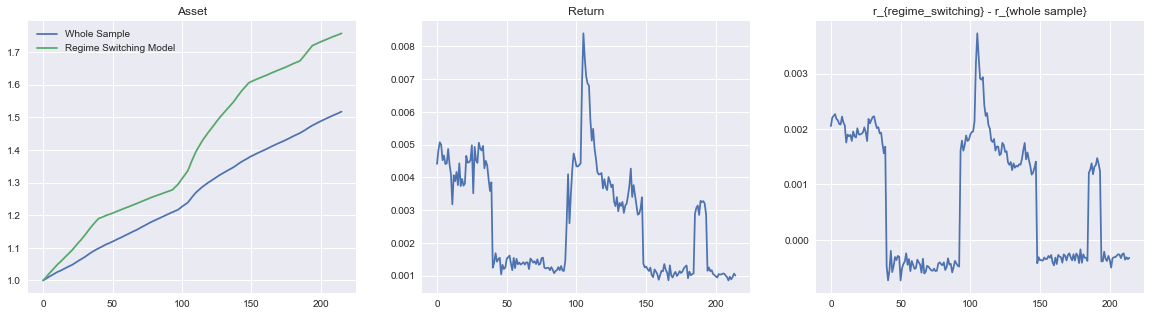
\includegraphics[width=16.5cm,height=5cm,angle=0]{BB.png}\\
\caption{Credit Portfolio for BB}
\end{figure}

Surprisingly, the regime switching model improve the performance for credit portfolio a lot, and the asset process is significantly increasing when separating market into different states. It means for the Junk Bond investors, they are more sensitive to the market environment, and we could make more profit with credit portfolio when bond are sensitive. Also, the sharp change of the return rate in the center diagram shows the volatile risk premium in BB bond. And the improvement of regime switching model is always positive in left diagram, which means the regime switching model can always improve our credit portfolio.

\subsection{CCC bond}
For CCC bond, the property of Junk Bond shows more significantly.
\begin{figure}[H]
\centering
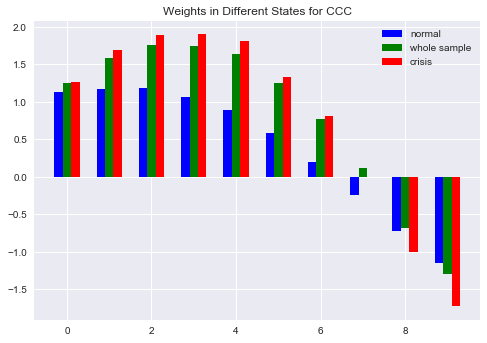
\includegraphics[width=16.5cm,height=6cm,angle=0]{CCC_weight.png}\\
\caption{Weights for bond in CCC}
\end{figure}
\begin{figure}[H]
\centering
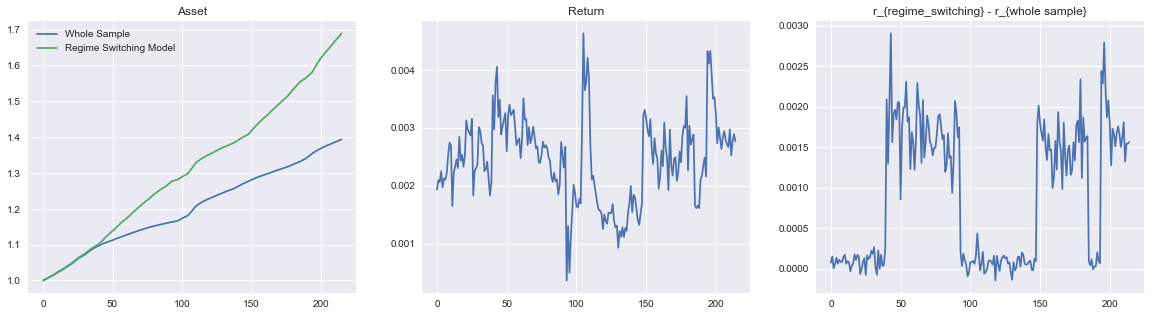
\includegraphics[width=16.5cm,height=5cm,angle=0]{CCC.png}\\
\caption{Credit Portfolio for CCC}
\end{figure}

It seems that regime switching model could improve more if the bond is more `junk', in other word, more sensitive to the market and more volatile. We can interpret this phenomenon that regime switching model could provide us with more accurate insights to the market regardless of the states. And it could improve more if the states are more different.\\

\subsection{Portfolio Evaluation}
From the credit portfolio constructed by AAA, BB and CCC bond , we have the results in the past decades below. We can assess the credit portfolio by average return and Sharpe Ratio.


\begin {table}[H]
\caption {Performance of Credit Portfolios} 
\label{tab:title} 
\begin{center}
\begin{tabular} {c c c c}
\hline\hline
Bond & AAA & BB & CCC \\
\hline

\multirow{Return} & 1.23\% & 3.15\% & 2.93\% \\

\multirow{Sharpe Ratio} & 1.85 & 1.60 & 3.36 \\

\hline\hline

\end{tabular}\\

\end{center}
\end {table}

Based on the Sharpe ratio, the return of credit portfolio shows a steady growth and good Sharpe Ratio, which benefits from steady yield of the bond and stabilized credit premium. But we need to choose our best portfolio between BB bond and CCC bond, for the reason that credit portfolio built on AAA bond possess relative low annually return, and we can get higher return as well as good Sharpe Ratio in BB bond and CCC bond.\\

Between BB and CCC, we prefer to choose the credit portfolio built on BB bond, for return dominates Sharpe Ratio when both of them are good enough. For the risk resource of bond portfolio, there are other risk except interest rate risk and credit risk, such as liquidity risk. So we could not perfectly catch the credit risk, and our portfolio may possess other risk. It means we'd better build our portfolio on relatively good bond and BB would be better than CCC.


\pagestyle{fancyplain}
\lhead{\fancyplain{}{\sf Mingcan, Lihua, Duo, Runsheng}}
\rhead{\fancyplain{}{\sf Summary}}
\cfoot{}

\section{Summary}
In this report, we firstly conduct regime switching model on GNP data and S\&P 500 Index, to get an insight about different states based on different data. We find that, compared with GNP data, S\&P is more sensitive to the market trend and accurate in identifying crisis. The GNP could only show the financial crisis in 2018, which is not enough for us to train our credit portfolio. But S\&P could even identify dot-com bubble collapse in 2000 and oil crisis in 2015, which is better for crisis detection.\\

Also, we apply PCA on the collections of Fama Bliss Yield and analyze the difference between the results of PCA with PCs major component. Then we use the PC1 and PC2 to do the statistical factor regression on high rating bond and low rating bond, checking if regime switching model could offer better understanding of the market. And we analyze the residual in different period to see the changes of credit risk in the past decades.\\

At last, we construct credit portfolio with the residual and intercept from the result of statistical factor regression. By comparing the effect of regime switching model and credit rating bonds, we find that the lower is credit rating, the better is the effect of regime switching model. And we evaluate different credit portfolio and choose the best credit portfolio built on BB bond.





\pagestyle{fancyplain}
\lhead{\fancyplain{}{\sf Mingcan, Lihua, Duo, Runsheng}}
\rhead{\fancyplain{}{\sf Appendix}}
\cfoot{}

\section{Appendix}

\begin {table}[H]
\caption {Maturities of the bond} \label{tab:title} 
\begin{center}
\begin{tabular} {|c|c|c|c|}
\hline
0 to 6 Month &  6 to 12 Month \\
\hline
12 to 18 Month & 18 to 24 Month\\
\hline
24 to 30 Month & 30 to 36 Month\\
\hline 
36 to 42 Month & 42 to 48 Month\\
\hline
48 to 54 Month & 54 to 60 Month\\
\hline
\end{tabular}\\
\end{center}
\end {table}

Variance Explanation in section 3

\begin{figure}[H]
\centering
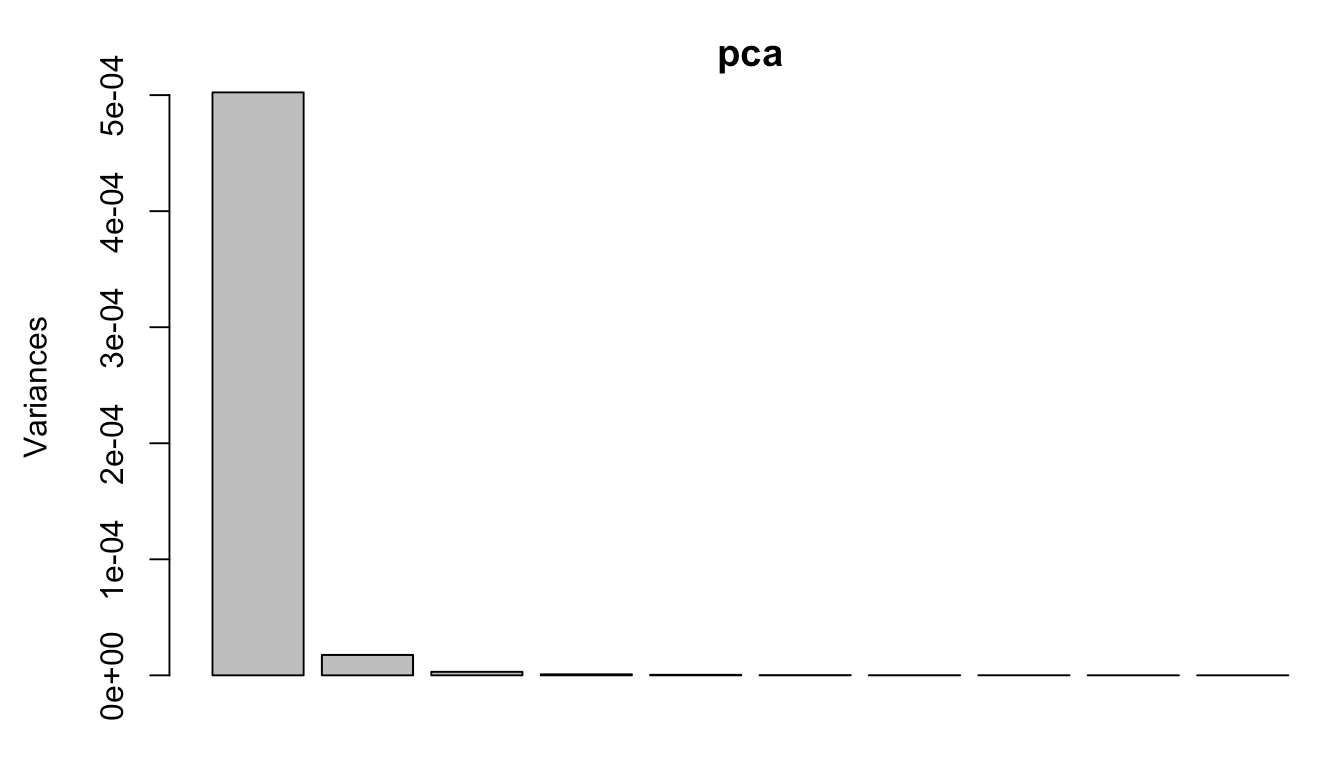
\includegraphics[width=16.5cm,height=6cm,angle=0]{2.png}\\
\caption{Variance Explanation for Full Period)}
\end{figure}

\begin{figure}[H]
\centering
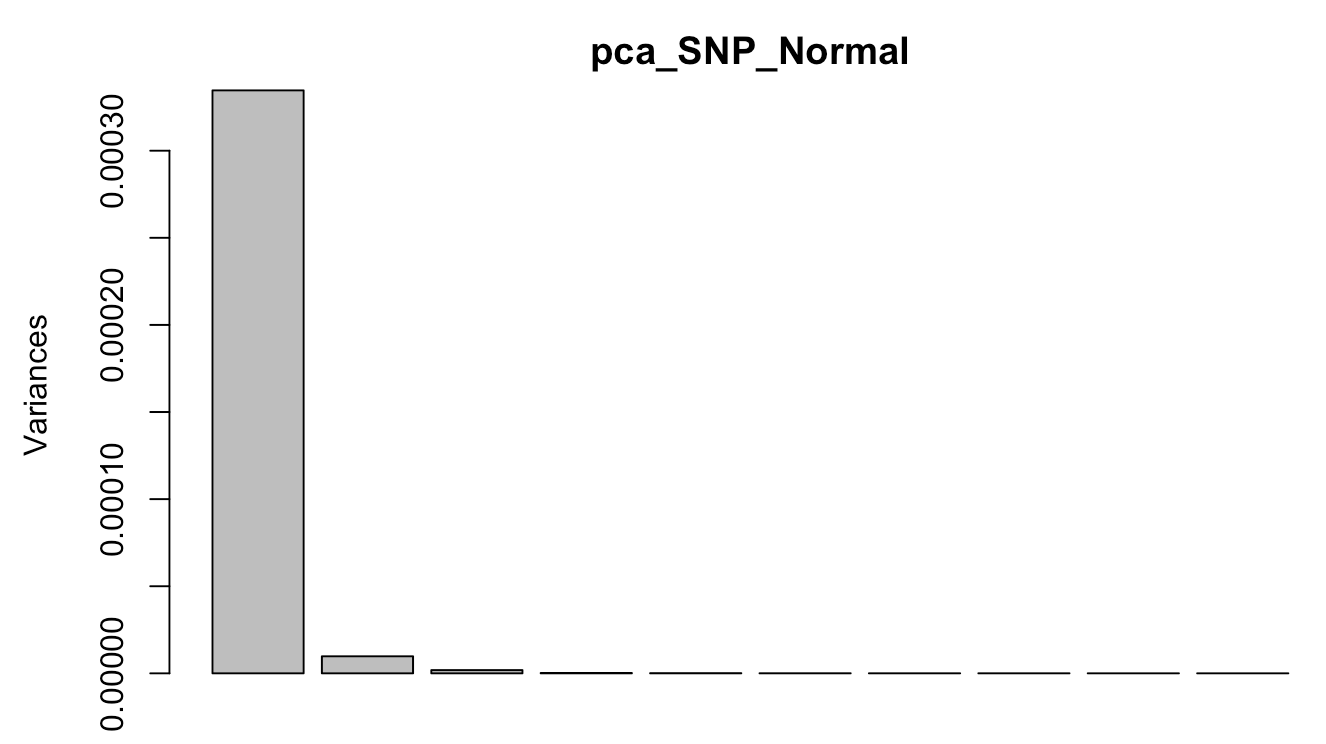
\includegraphics[width=16.5cm,height=6cm,angle=0]{11.png}\\
\caption{Variance Explanation for Crisis State}
\end{figure}

\begin{figure}[H]
\centering
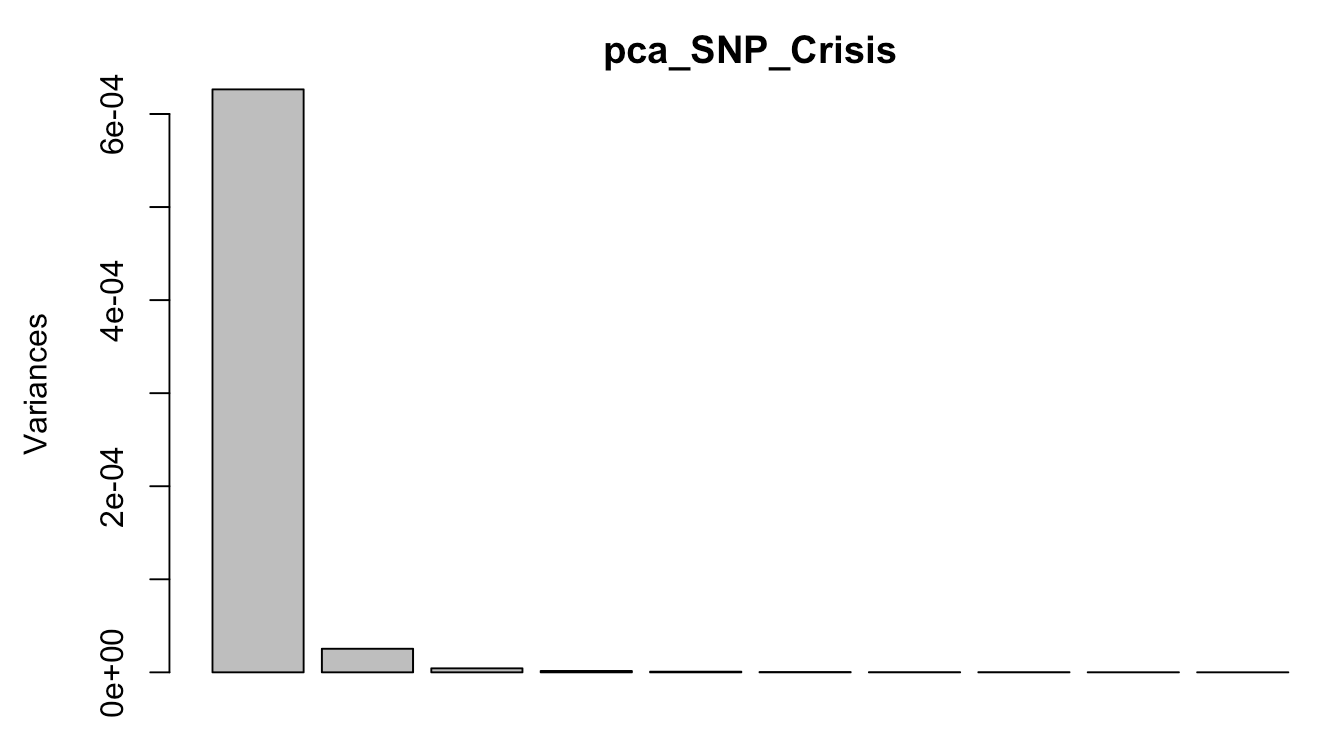
\includegraphics[width=16.5cm,height=6cm,angle=0]{14.png}\\
\caption{Variance Explanation for Normal State}
\end{figure}

The auto-correlation and normality tests of the residuals in the section 5:

\begin{figure}[H]
\centering
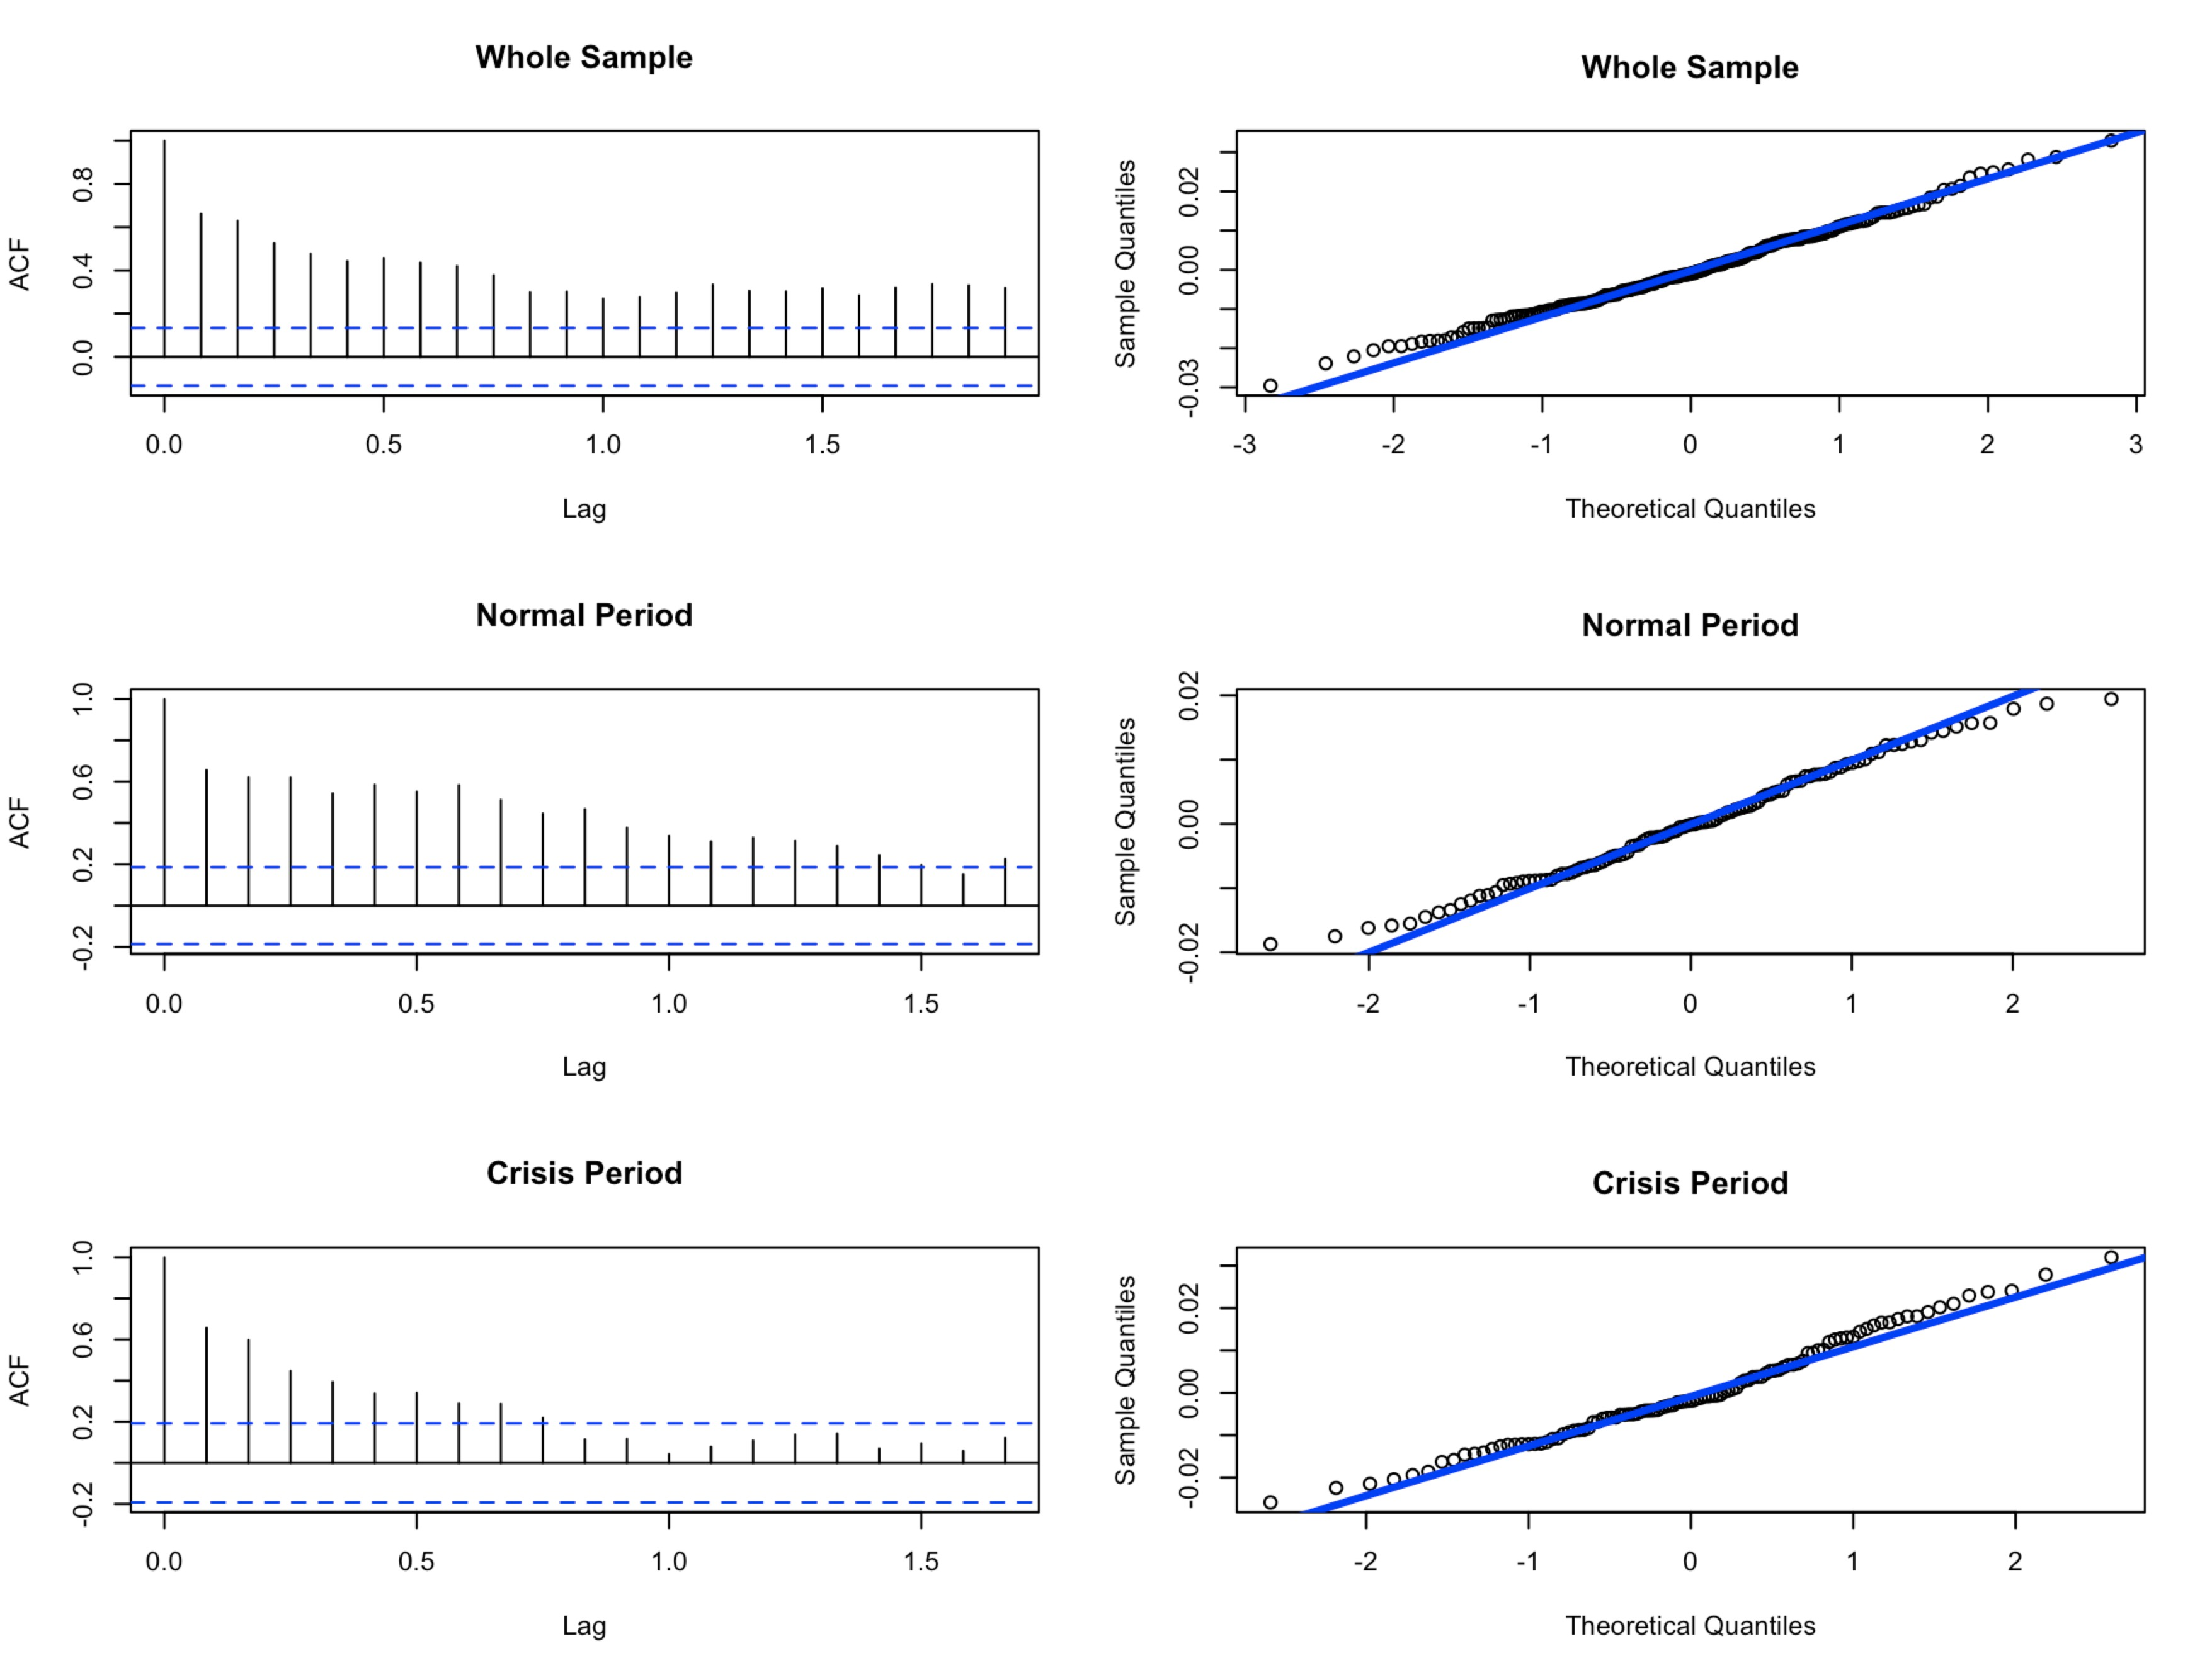
\includegraphics[width=15cm,height=13cm,angle=0]{AAA_resid_tests.jpg}\\
\caption{AAA Bond Residual Tests}
\end{figure}


\begin{figure}[H]
\centering
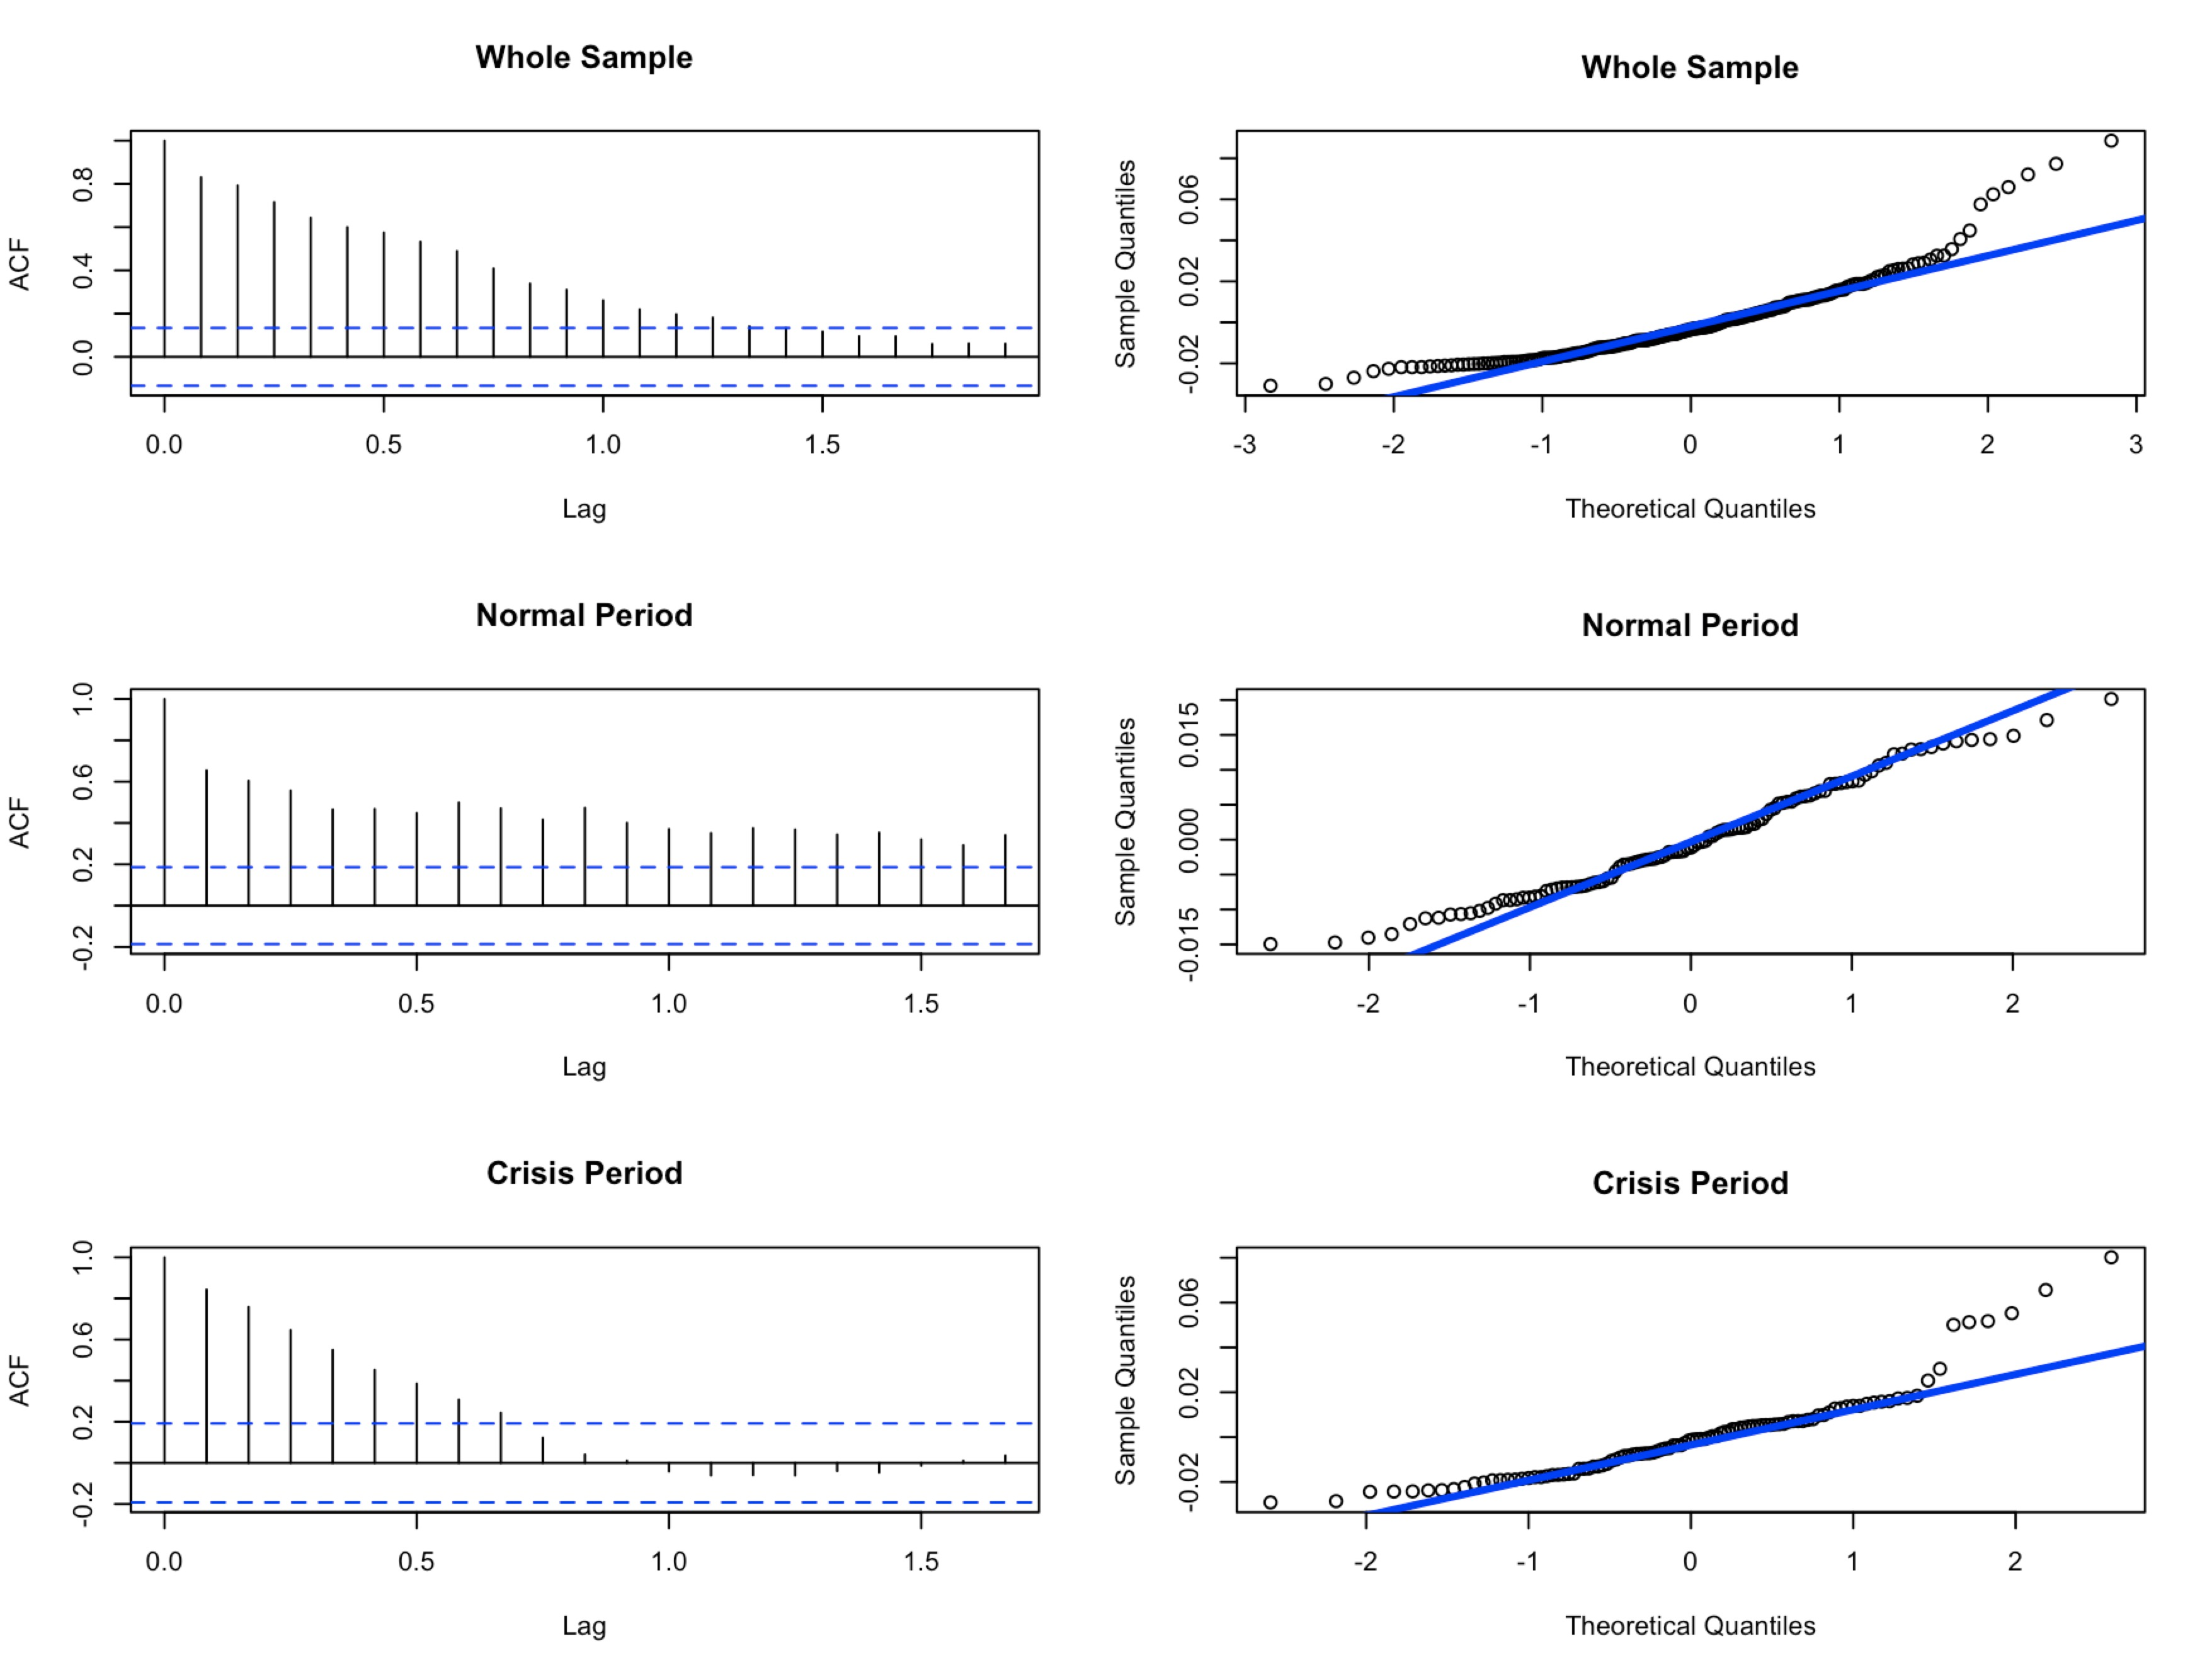
\includegraphics[width=15cm,height=13cm,angle=0]{BB_resid_tests.jpg}\\
\caption{BB Bond Residual Tests}
\end{figure}


\begin{figure}[H]
\centering
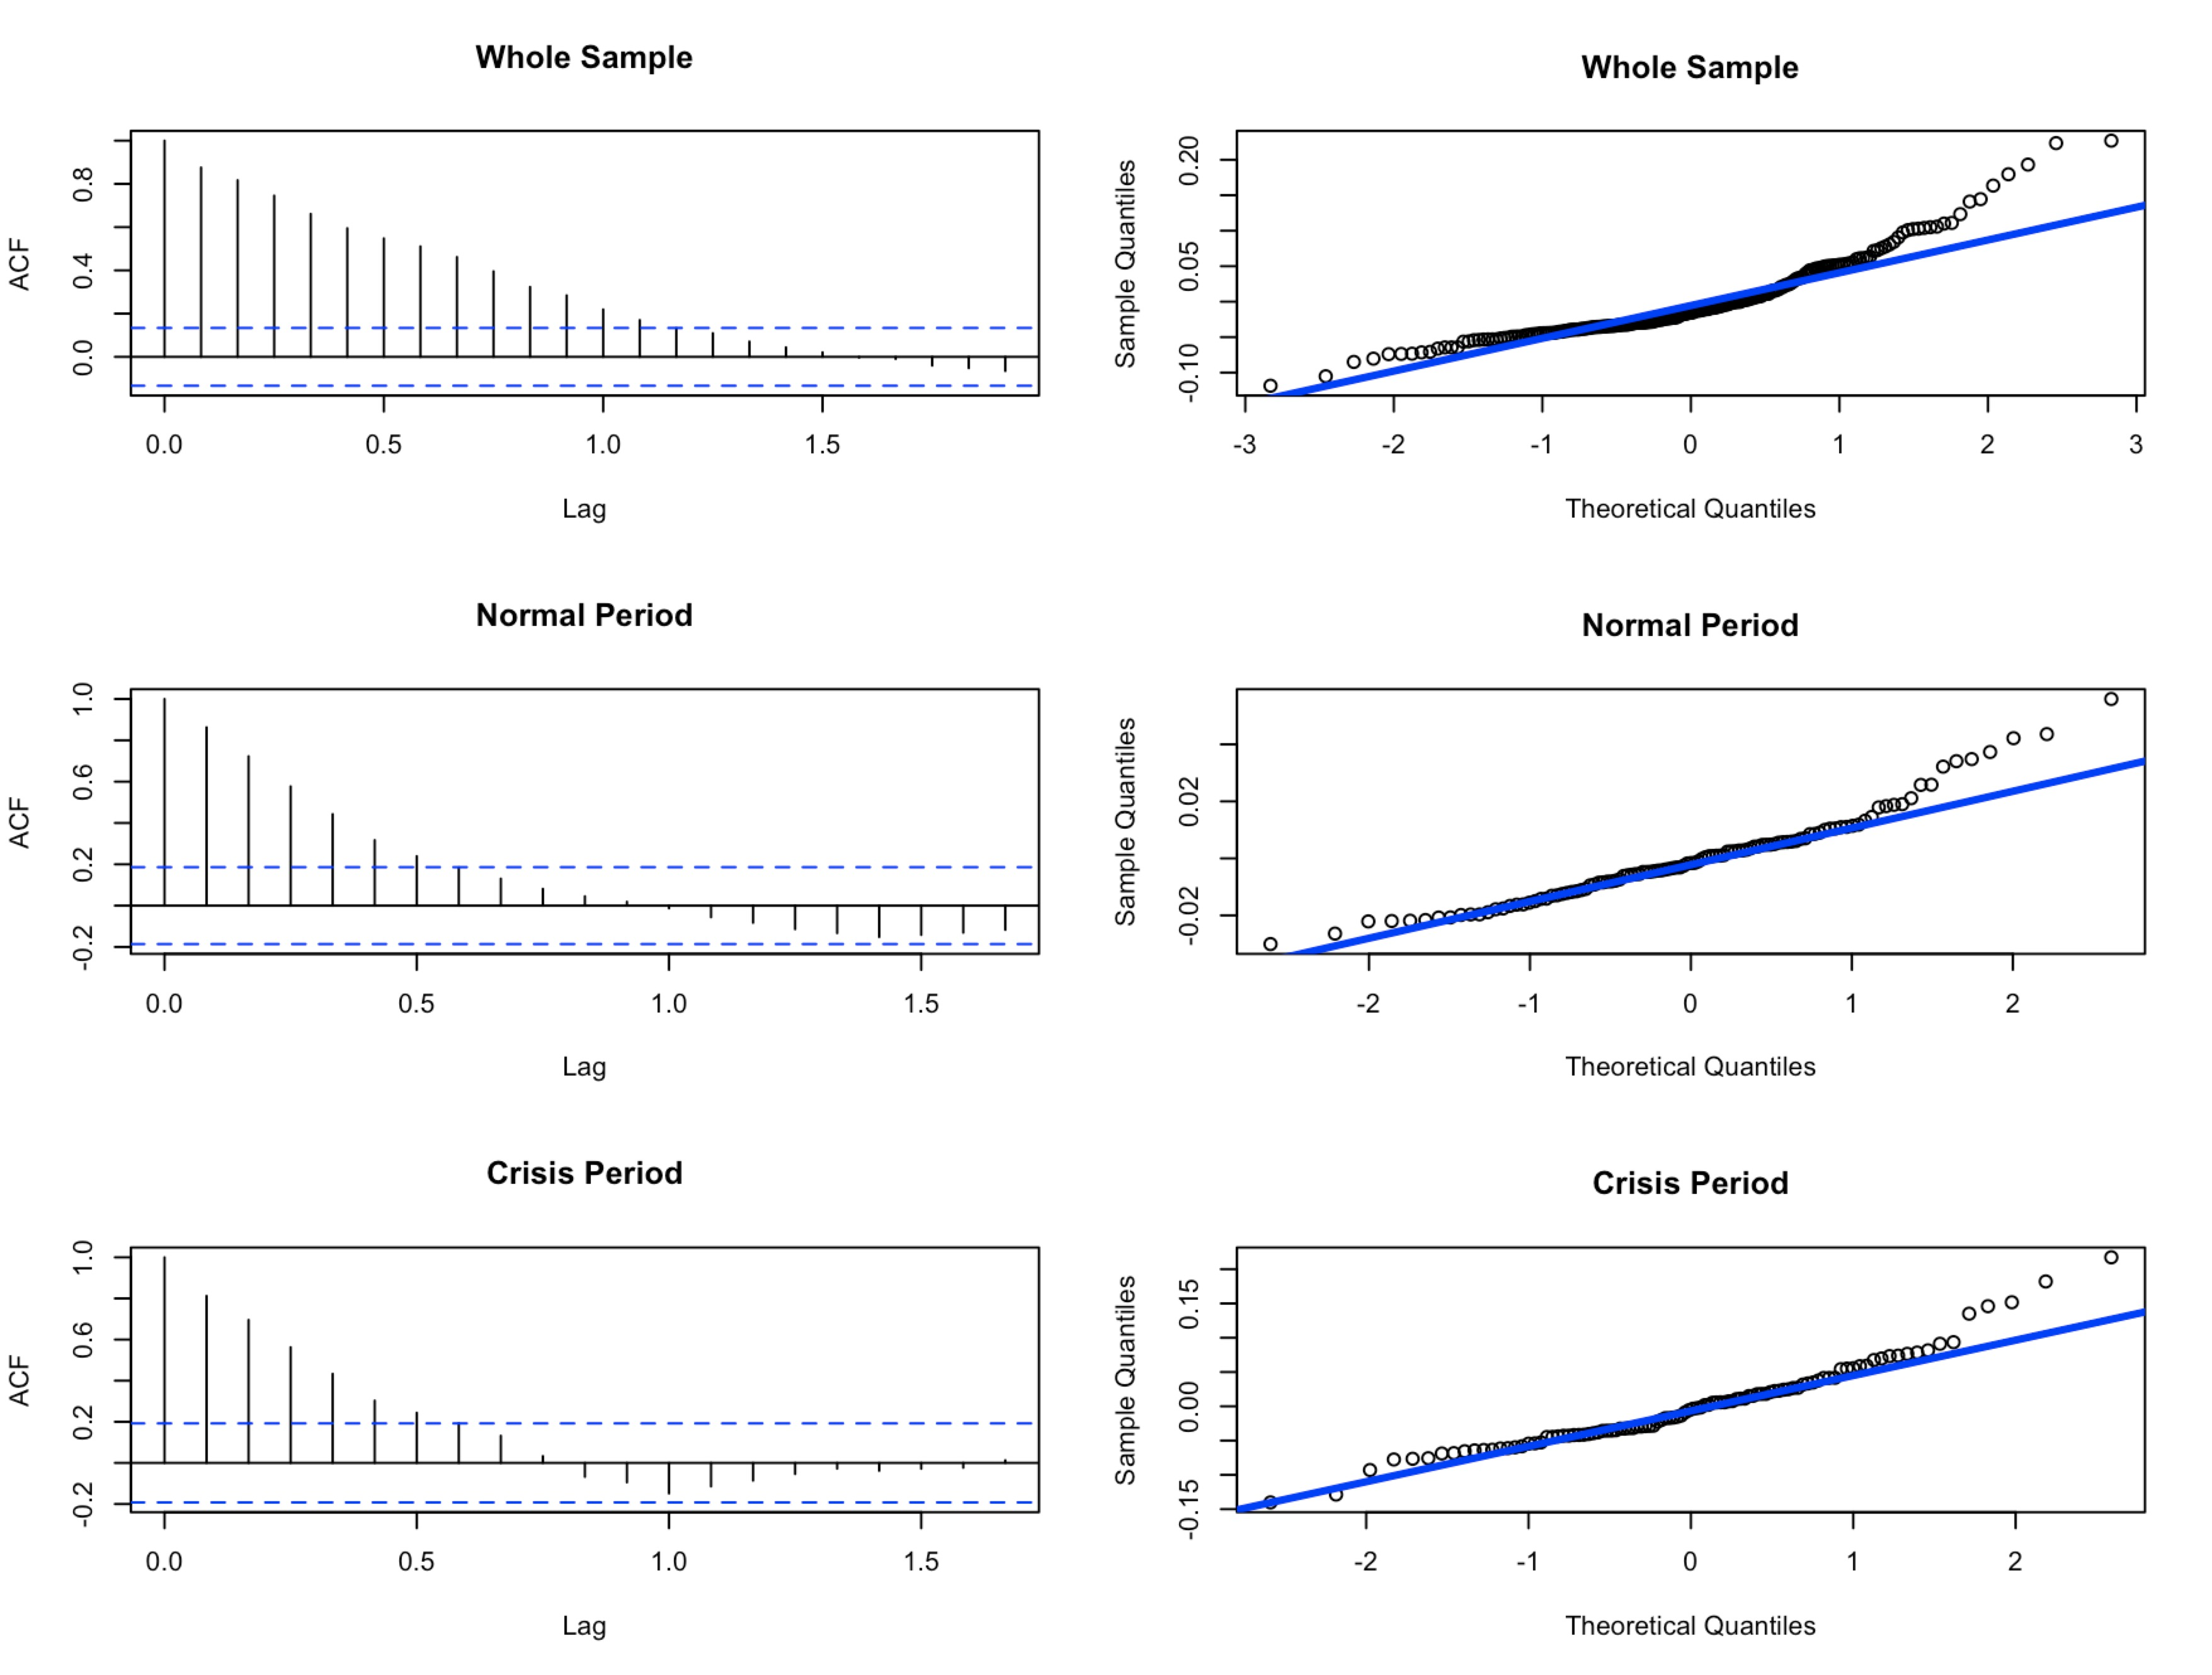
\includegraphics[width=15cm,height=13cm,angle=0]{CCC_resid_tests.jpg}\\
\caption{CCC Bond Residual Tests}
\end{figure}

\begin{figure}[H]
\centering
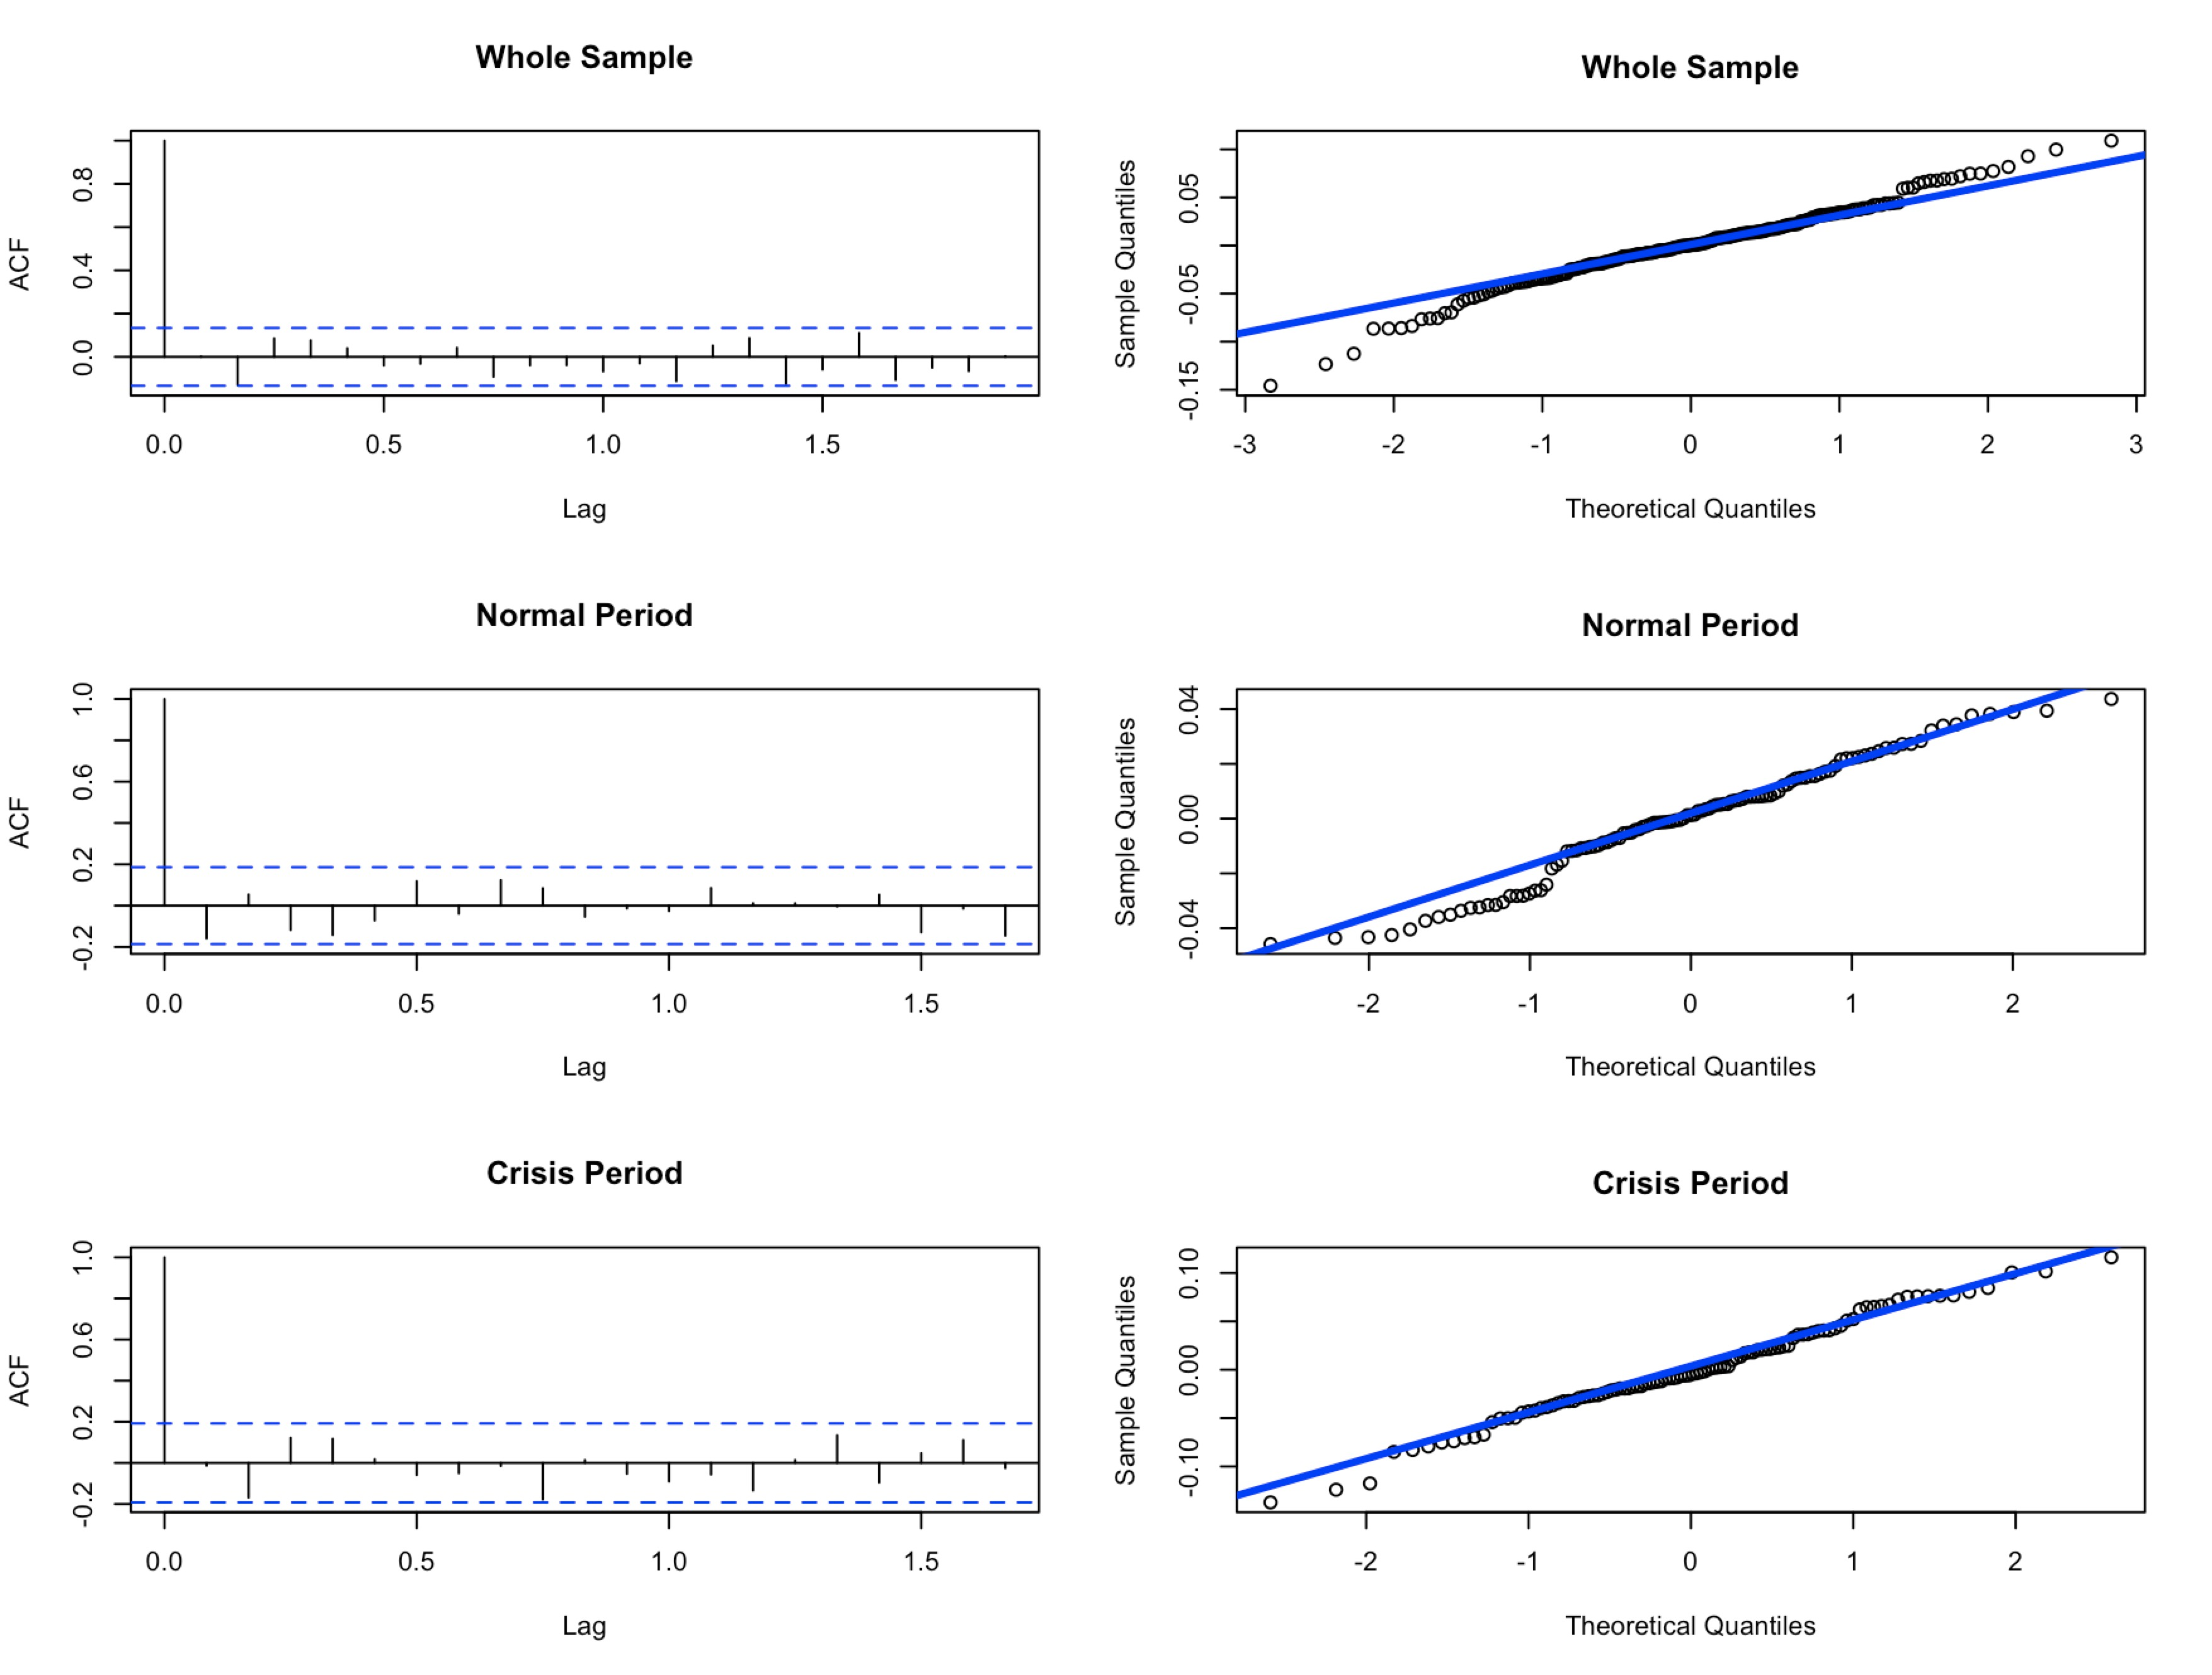
\includegraphics[width=15cm,height=13cm,angle=0]{s&p500_resid_tests.jpg}\\
\caption{CCC Bond Residual Tests}
\end{figure}



\end{document}












